\documentclass[
    a4paper,        % Papierformat
    11pt,           % Schriftgröße
    ngerman,        % Sprache für Trennung und Bezeichnungen
    parskip=half,   % Halbe Zeile Abstand zwischen Absätzen (statt Einrücken)
    listof=totoc,   % Abbildungs-/Tabellenverzeichnis im Inhaltsverzeichnis
    bibliography=totoc % Literaturverzeichnis im Inhaltsverzeichnis
]{scrartcl}

% --- Grundlegende Pakete ---
\usepackage[utf8]{inputenc} % Kodierung (bei modernen Editoren oft Standard)
\usepackage[T1]{fontenc}    % Wichtig für Umlaute und Trennung
\usepackage{lmodern}        % Schöneres Schriftbild (Vektorschrift)
\usepackage{babel}          % Deutsche Bezeichnungen (Inhaltsverzeichnis etc.)

% --- Mathe und Technik ---
\usepackage{amsmath, amssymb, amsthm, nicefrac} % Mathematische Formeln
\usepackage{siunitx}        % WICHTIG für Einheiten: \SI{5}{\meter}
\sisetup{locale = DE}       % Komma statt Punkt als Dezimaltrenner

% --- Grafik und Tabellen ---
\usepackage{graphicx}       % Einbinden von Bildern
\usepackage{booktabs}       % Schönere Tabellenlinien (\toprule, \midrule, \bottomrule)
\usepackage{float}          % Um Bilder an exakten Stellen zu platzieren [H]
% --- Design und Layout ---
\usepackage[left=2.5cm, right=2.5cm, top=2.5cm, bottom=2.5cm]{geometry} % Ränder
\usepackage[headsepline]{scrlayer-scrpage} % Kopf- und Fußzeilen
\pagestyle{scrheadings}
\clearpairofpagestyles
\ihead{} % Kopfzeile links
\ohead{\today}              % Kopfzeile rechts
\cfoot{\pagemark}           % Seitenzahl unten mitte

% --- Verlinkungen (sollte meist als letztes geladen werden) ---
\usepackage[hidelinks]{hyperref} % Klickbare Links im PDF, keine roten Rahmen

\usepackage{listings}
\usepackage{xcolor}
\graphicspath{{Images/}}

% Einfache Konfiguration für Python-Optik
\lstset{
    language=Python,
    basicstyle=\ttfamily\small,
    keywordstyle=\color{blue},
    commentstyle=\color{green!50!black},
    stringstyle=\color{orange},
    numbers=left,
    numberstyle=\tiny,
    frame=single,
    breaklines=true,
    captionpos=b
}
\begin{document}

% ==========================================
% DECKBLATT
% ==========================================
\begin{titlepage}
    \centering
    % Platzhalter für ein Logo (auskommentieren, wenn Bild vorhanden)
    % \includegraphics[width=0.4\textwidth]{logo.png} 
    \vspace{2cm}
    
    {\scshape\LARGE Hochschule Karlsruhe \par}
    \vspace{1cm}
    {\scshape\Large Fakultät für Maschinenbau \& Mechatronik \par}
    {\scshape\Large Studiengang Robotik und KI in der Produktion \par}
    \vspace{1.5cm}
    
    {\huge\bfseries Projektbericht zum Fach Künstliche Intelligenz \par}
    \vspace{0.5cm}
    {\Large Erkennung von QR-Codes \par}
    
    \vspace{2cm}
    
    % Autoren in einer Tabelle nebeneinander
    \vspace{2cm}
    \begin{center}
        \begin{tabular}{l p{2cm} l}
            Marlon Leitschuh    & & Nico Sander \\
            Matrikelnr: 103626  & & Matrikelnr: 74808 \\
            lema1046@h-ka.de    & & sani1019@email.de \\
        \end{tabular}
    \end{center}

    \vfil

    \textbf{Betreuung:} \\
    Prof. Dr. -Ing. habil. Catherina Burghart

    \vspace{0.8cm}
    
    \textbf{Datum:} \\
    \today
    
\end{titlepage}

% ==========================================
% VERZEICHNISSE
% ==========================================
\tableofcontents            % Inhaltsverzeichnis
\newpage

% ==========================================
% INHALT
% ==========================================

\section{Einleitung}

Zur Steuerung des Waschprozesses und der gewählten Zusatzoptionen gibt die Waschanlage einen Beleg mit QR-Code aus, welcher hinter der Windschutzscheibe zu positionieren ist. Eine zentrale Anforderung an das System ist die kontinuierliche Erfassung dieses Codes durch eine Kamera, sowohl vor als auch während des Waschvorgangs. Die Lesbarkeit muss hierbei auch unter erschwerten Bedingungen, etwa durch Verschmutzungen, Nässe oder Schaumbildung auf der Scheibe, gewährleistet sein. Des Weiteren ist zu berücksichtigen, dass sich im Sichtfeld potenziell diverse Störobjekte oder weitere Schriftstücke (mit oder ohne QR-Codes) befinden können.
%
\subsection{Aufgabenstellung}

\subsubsection{Klassifikation}

Ein Kernziel ist die Entwicklung von Klassifikationsmodellen zur binären Unterscheidung, ob ein Bild einen QR-Code enthält (Klasse 1) oder nicht (Klasse 0). Als Datengrundlage ist zunächst eine umfangreiche Sammlung von Trainingsbildern erforderlich, welche eine hohe Varianz an realen Szenarien abdeckt. Durch eine gezielte Vorverarbeitung (Preprocessing) wird anschließend die notwendige Datenqualität für den Lernprozess sichergestellt.

Methodisch werden sowohl eine eigenständige Modellarchitektur als auch drei Ansätze des Transfer-Learnings implementiert. Diese Modelle gilt es zu trainieren und durch die systematische Variation der Hyperparameter so lange zu optimieren, bis Leistung zufriedenstellend ist.

\subsubsection{Detektion, Decodierung und geometrische Analyse}

In diesem Arbeitsschritt ist das System von einer reinen Bildklassifikation zu einer Objektdetektion zu erweitern. Während die Klassifikation lediglich das Vorhandensein eines QR-Codes im Gesamtbild bestätigt, zielt die Detektion darauf ab, die exakten Koordinaten (Bounding Box) des Codes innerhalb des Bildes zu lokalisieren.

Auf Basis dieser Lokalisierung sind folgende Teilaufgaben zu implementieren:
\begin{enumerate}
    \item \textbf{Verifikation der Lesbarkeit:} Die detektierten Bildbereiche sind an einen QR-Code-Scanner zu übergeben. Das Ergebnis ist visuell im Ausgabebild zu kennzeichnen: Erfolgreich decodierbare Codes sind mit einem grünen Rahmen zu versehen, während detektierte, aber nicht lesbare Objekte rot zu markieren sind.
    \item \textbf{Winkelberechnung:} Anhand der geometrischen Verzerrung des erkannten Codes ist eine Stellgröße für die Kamerahardware zu ermitteln. Es ist zu berechnen, um wie viel Grad eine darüber montierte Kamera (ausgehend von einer planparallelen Ausrichtung zum Boden) geschwenkt werden muss, um eine optimale Erfassung zu gewährleisten.
\end{enumerate}

\subsection{Herausforderungen}
Die Umsetzung des Systems unterliegt mehreren spezifischen Herausforderungen, die sich aus den realen Einsatzbedingungen in einer Waschanlage ergeben:

\begin{itemize}
    \item \textbf{Variable Umgebungsbedingungen:} Die zuverlässige optische Erfassung wird durch den Zustand der Windschutzscheibe maßgeblich erschwert. Hierbei stellen Nässe, Seifenrückstände sowie starke Verschmutzungen signifikante Störfaktoren für die Bildverarbeitung dar.
    \item \textbf{Visuelle Störgrößen:} Das Sichtfeld der Kamera enthält neben dem relevanten QR-Code potenziell diverse Interferenzen. Hierzu zählen weitere Zettel, Objekte im Fahrzeuginnenraum sowie Spiegelungen auf der Glasoberfläche, die zu Fehlerkennungen führen können.
    \item \textbf{Erfassungsreichweite:} Die Auflösung und Detektionsleistung des Systems muss so ausgelegt sein, dass eine Identifikation des Codes auch aus einer Distanz von bis zu \SI{3}{\meter} sichergestellt ist.
\end{itemize}

\subsection{Ansatz}

Um die in der Aufgabenstellung beschriebenen Herausforderungen zu bewältigen, wurde ein Ansatz gewählt, der auf dem \textit{Sliding Window}-Verfahren basiert. Anstatt das gesamte Kamerabild in einem Schritt zu analysieren, wird das Bild in kleinere Teilbereiche zerlegt. Diese sogenannten Patches werden anschließend einzeln durch ein Klassifikationsmodell bewertet.

\subsubsection{Sliding Window Verfahren und Auflösungsunabhängigkeit}
Die Entscheidung für ein Sliding Window resultiert primär aus dem Missverhältnis zwischen der Gesamtbildgröße und der Größe des zu erkennenden Objekts. Da der QR-Code je nach Fahrzeugposition nur einen Bruchteil der Bildfläche einnimmt, würde eine einfache Skalierung des Gesamtbildes auf die Eingabegröße des neuronalen Netzes zu einem massiven Informationsverlust führen. Ein QR-Code, der im Originalbild nur wenige Pixel einnimmt, wäre nach der Komprimierung nicht mehr von Störrauschen zu unterscheiden.

Durch das Sliding Window bleibt die ursprüngliche Detailtiefe in den Ausschnitten erhalten. Das Fenster gleitet mit einer definierten Schrittweite über das Bild und extrahiert potenzielle Kandidatenbereiche. Dies bietet den Vorteil, dass Störfaktoren wie andere Schriftstücke oder Spiegelungen isoliert betrachtet werden können.

Ein weiterer wesentlicher Vorteil dieser Implementierung ist die Robustheit gegenüber unterschiedlichen Kameraauflösungen. Da die Größe des gleitenden Fensters nicht statisch in Pixeln, sondern relativ zu den Dimensionen des Eingabebildes definiert wird, passt sich das System dynamisch an. Das Verfahren funktioniert somit gleichermaßen für Bilder in Full-HD ($1920 \times 1080$ Pixel) wie für hochauflösende 4K-Aufnahmen, ohne dass eine manuelle Anpassung der Parameter erforderlich ist.

\subsubsection{Skalenunabhängigkeit (Multi-Scale Ansatz)}
Eine besondere Herausforderung dieses Projekts ist die variable Distanz von bis zu \SI{3}{\meter}. Ein QR-Code kann dadurch im Kamerabild sehr groß oder sehr klein erscheinen. Ein starres Fenster fester Größe würde hier nicht ausreichen.

Unsere Implementierung löst dies durch einen dynamischen Multi-Scale-Ansatz. Das System iteriert in mehreren Durchläufen über das Bild und verwendet dabei jeweils unterschiedliche Fenstergrößen, die als Bruchteil der Bildkante definiert sind (z.\,B. $\nicefrac{1}{2}, \nicefrac{1}{3}$ oder $\nicefrac{1}{4}$ der Bildgröße). Jeder ausgeschnittene Bereich wird anschließend auf die einheitliche Zielgröße des neuronalen Netzes skaliert.

Dadurch erreichen wir eine Unabhängigkeit von der physischen Entfernung:
\begin{itemize}
    \item Ein naher, großer QR-Code wird durch ein großes Fenster (z.\,B. $\nicefrac{1}{2}$) optimal erfasst.
    \item Ein ferner, kleiner QR-Code wird durch ein kleines Fenster (z.\,B. $\nicefrac{1}{8}$) präzise ausgeschnitten.
\end{itemize}
Für das neuronale Netz sehen nach der Skalierung beide Fälle identisch aus. Es lernt somit abstrakte Merkmale eines QR-Codes, unabhängig davon, wie viel Platz dieser im ursprünglichen Gesamtbild eingenommen hat.

\subsubsection{Verbindung von Klassifikation und Detektion}
Obwohl wir primär Klassifikationsmodelle trainieren, ermöglicht dieser Ansatz bereits eine implizite Objektdetektion. Klassische Klassifikation beantwortet nur die Frage nach dem Vorhandensein eines QR-Codes im Bild. Durch die Zerlegung in Fenster beantworten wir jedoch die Frage, ob ein QR-Code in einem spezifischen Ausschnitt (Patch) zu finden ist.

Da die Koordinaten $(x, y)$ jedes Fensters während der Generierung bekannt sind, liefert eine positive Klassifikation automatisch eine räumliche Verortung. Dies bildet die Grundlage für die spätere Heatmap-Erstellung und die Extraktion der Bounding Box. Komplexe Detektions-Architekturen wie YOLO sind somit für diesen Schritt nicht zwingend erforderlich.

\section{Daten}

\subsection{Datenerhebung}

\subsection{Vorverarbeitung \& Labeling}

\subsection{Datenaugmentation}

\subsection{Finaler Datensatz}

\section{Netzarchitekturen}

\subsection{Experimentelle Entwicklung}

\subsection{Finales Modell}

\section{Transfer Learning}

\subsection{MobileNetV3Small}

\subsubsection{Experimentelle Entwicklung}

\subsubsection{Finales Modell}

\subsection{MobileNetV2}

\subsubsection{Experimentelle Entwicklung}

\subsubsection{Finales Modell}

\subsection{EfficientNetB0}

\subsubsection{Experimentelle Entwicklung}

\subsubsection{Finales Modell}

% ==========================================
% KAPITEL 5: INFERENZ
% ==========================================
\section{Inferenz}

Die Inferenzphase stellt den operativen Kern des Systems dar. In diesem Schritt wird das trainierte Modell eingesetzt, um auf neuen, unbekannten Bildern Vorhersagen zu treffen. Da die QR-Codes im Verhältnis zur Gesamtauflösung der Kamera oft nur eine sehr kleine Fläche einnehmen, ist eine direkte Klassifikation des Gesamtbildes nicht zielführend.

Der Prozess folgt einer mehrstufigen Pipeline: Zunächst wird das Bild durch ein Sliding-Window-Verfahren vorverarbeitet. Dieser Schritt ist identisch mit dem Verfahren zur Generierung der Trainingsdaten, was eine konsistente Merkmalsextraktion über alle Projektphasen hinweg sicherstellt. Die extrahierten Bildbereiche (Patches) werden einzeln bewertet und die Resultate anschließend in einer Heatmap fusioniert, um die exakte Position der auf dem Gesamtbild für die nachfolgende Decodierung zu bestimmen.

\begin{figure}[H]
    \centering
    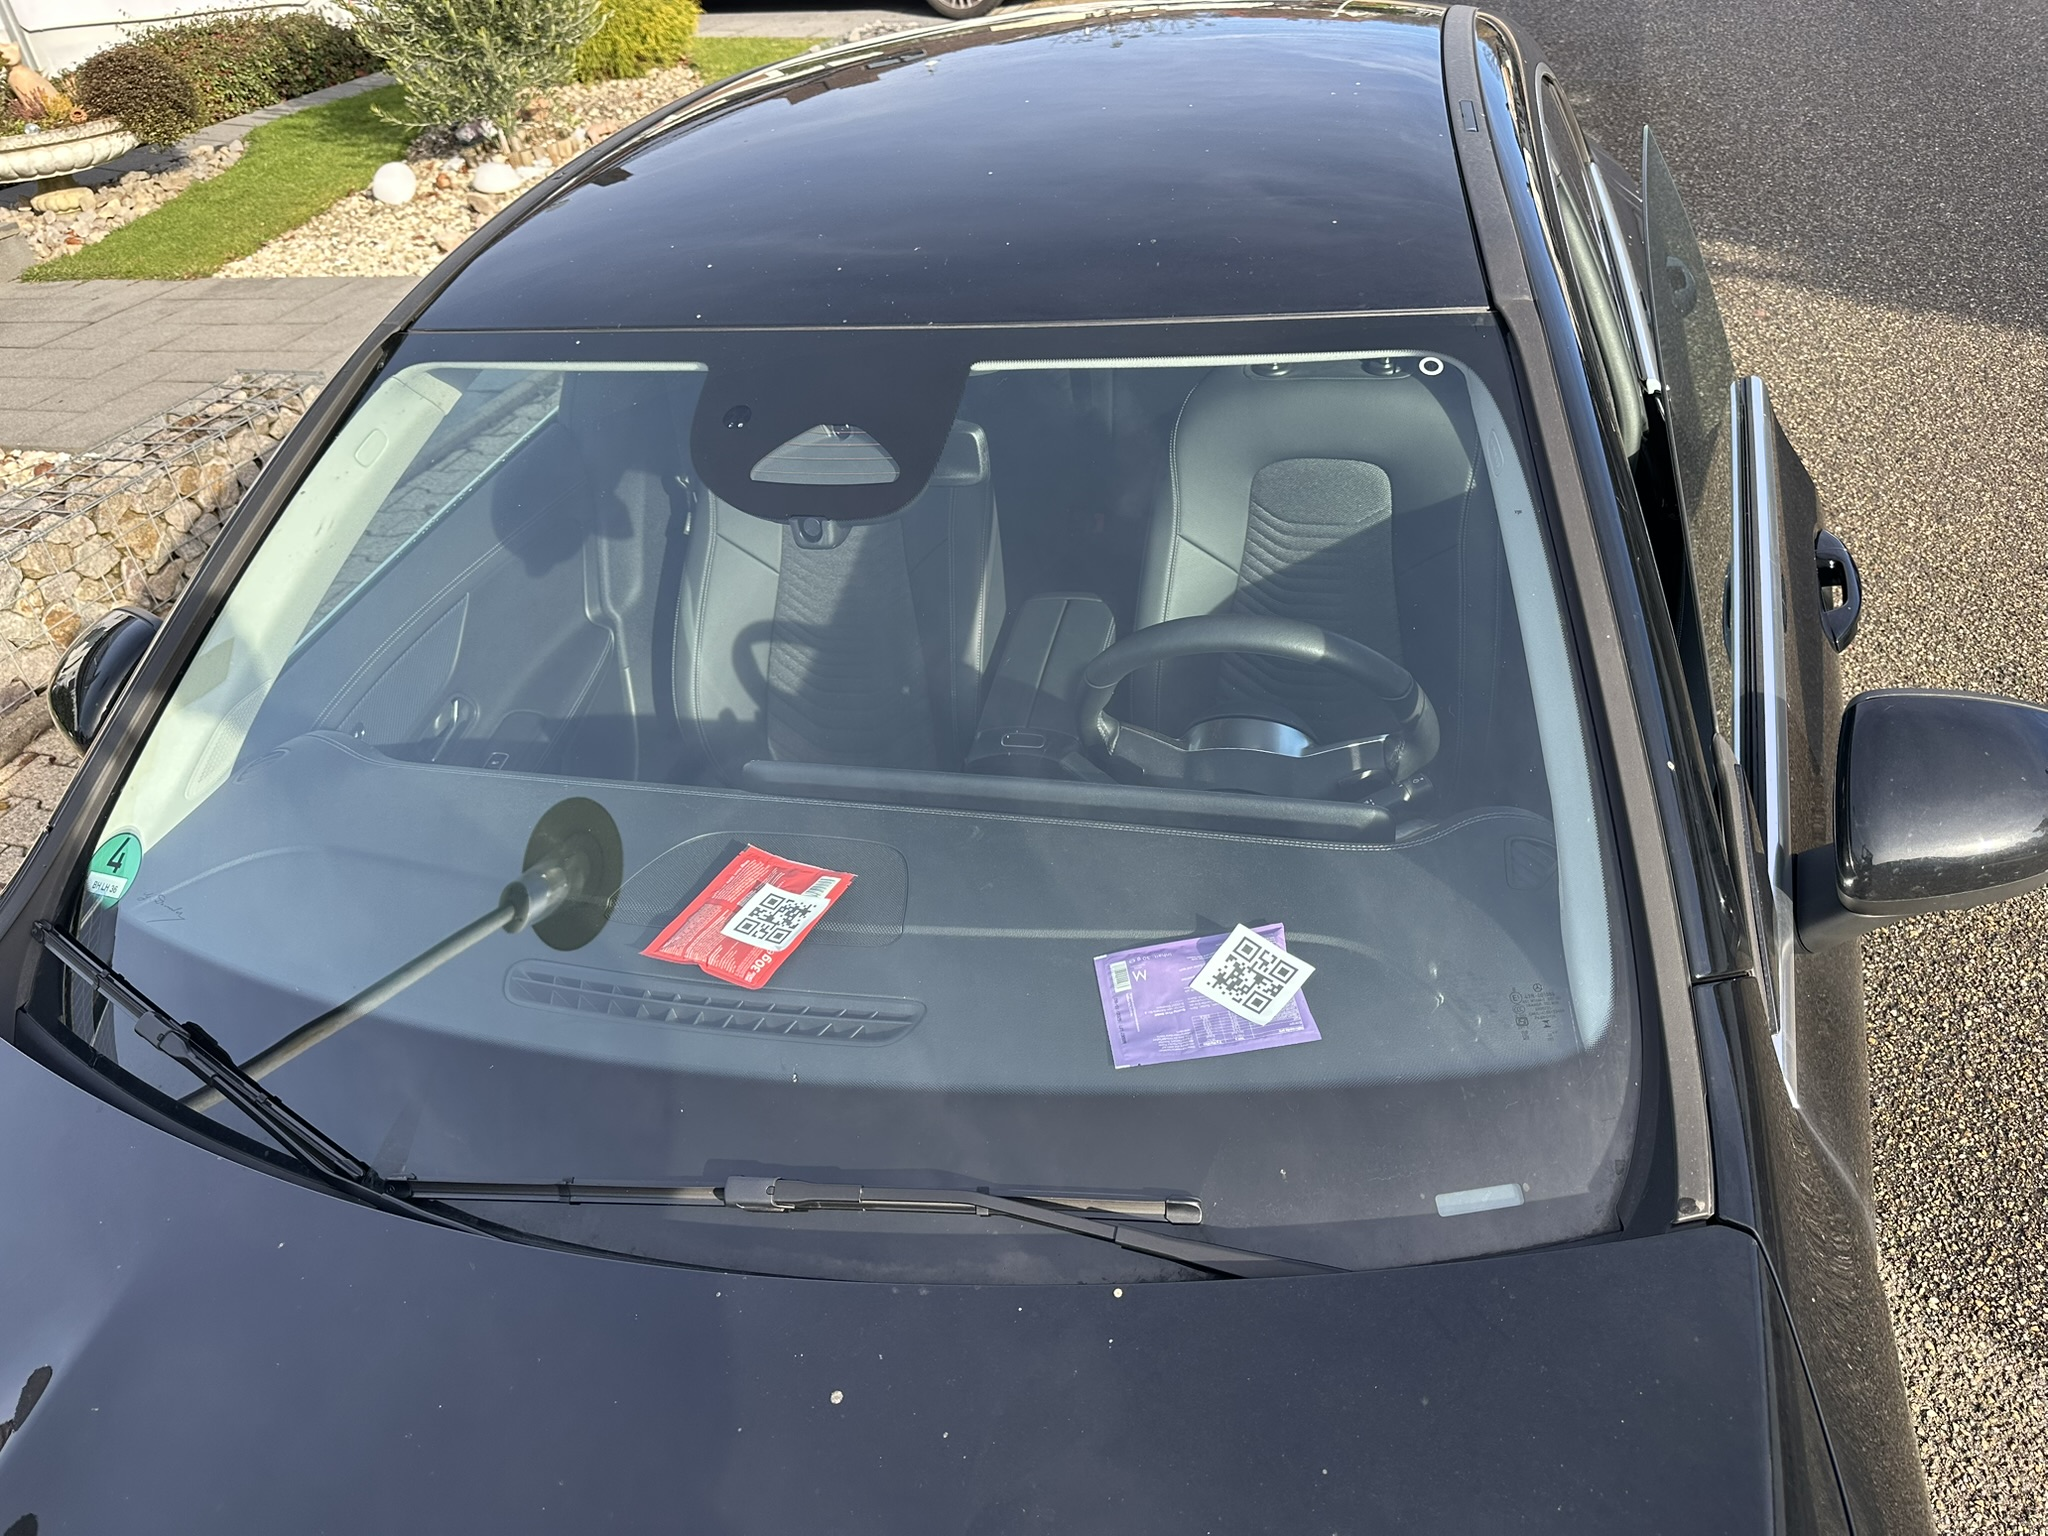
\includegraphics[width=0.8\textwidth]{Originalbild.png}
    \caption{Beispiel zur Analyse}
    \label{fig:patch_example}
\end{figure}


\subsection{Vorverarbeitung: Multi-Scale Sliding Window}

Um der Herausforderung variabler Distanzen von bis zu \SI{3}{\meter} zu begegnen, wird ein patch-basierter Ansatz gewählt. Anstatt das Bild pauschal zu skalieren und dabei kritische Details zu verlieren, gleitet ein virtuelles Fenster über die Aufnahme. Durch die Verwendung verschiedener Skalierungsfaktoren wird eine Skaleninvarianz erreicht, die es ermöglicht, QR-Codes unabhängig von ihrer physischen Entfernung zur Kamera in einer optimalen Auflösung zu erfassen.

\subsubsection{Implementierung und Konfiguration}

Die technische Umsetzung erfolgt über eine zentrale Konfigurationsstruktur, welche die Dynamik des Fensters steuert. Der folgende Code-Ausschnitt zeigt die im Projekt verwendete Konfiguration:

\begin{lstlisting}[language=Python, caption={Konfiguration der Sliding Window Parameter}]
@dataclass
class MultiScaleConfig:
    patch_size: int = 256
    scale_divisors: list = [1.5, 2.0, 3.0, 4.0, 6.0, 8.0]
    overlap: float = 0.5 
    use_relative_min_size: bool = True
    min_relative_factor: float = 0.15
    absolute_pixel_floor: int = 128
    interpolation: int = cv2.INTER_AREA
\end{lstlisting}

\subsubsection{Analyse der Einstellparameter}

Die Effizienz der Detektion hängt maßgeblich von der Justierung dieser Parameter ab:

\begin{table}[H]
    \centering
    \caption{Erläuterung der Sliding-Window-Parameter}
    \begin{tabular}{l p{9cm}}
        \toprule
        \textbf{Parameter} & \textbf{Funktion und Auswirkung} \\
        \midrule
        \texttt{patch\_size} & Definiert die quadratische Zielgröße (256 Pixel), auf die jeder Ausschnitt skaliert wird. \\
        \texttt{scale\_divisors} & Bestimmt die Skalierungsstufen. Kleine Divisoren finden nahe Objekte, große Faktoren isolieren weit entfernte QR-Codes. \\
        \texttt{overlap} & Regelt die Überlappung benachbarter Fenster (\SI{50}{\percent}). Dies stellt sicher, dass Objekte an den Schnittkanten zweier Fenster lückenlos erfasst werden. \\
        \texttt{min\_relative\_factor} & Definiert eine minimale Fenstergröße relativ zur Bildkante, um bei sehr hohen Auflösungen die Erzeugung informationsloser Patches zu verhindern. \\
        \texttt{interpolation} & Nutzt \texttt{cv2.INTER\_AREA}, was beim Verkleinern von Bildbereichen die beste Bildqualität liefert. \\
        \bottomrule
    \end{tabular}
\end{table}

\begin{figure}[H]
    \centering
    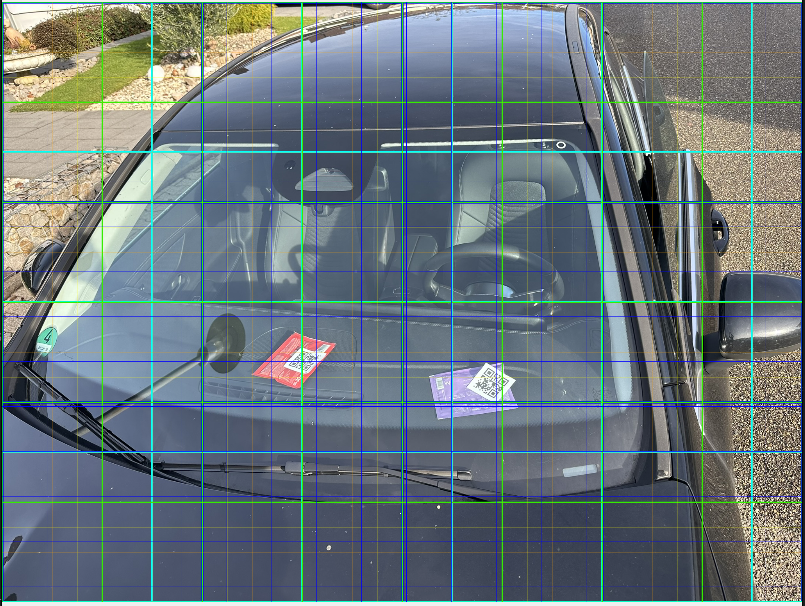
\includegraphics[width=0.8\textwidth]{SlidingWindows.png}
    \caption{Visualisierung des Sliding-Window-Rasters über verschiedene Skalierungsstufen hinweg.}
    \label{fig:sliding_window_grid}
\end{figure}

Die farbigen Gitterlinien in Abbildung \ref{fig:sliding_window_grid} markieren die Grenzen der extrahierten \textbf{Patches}. Jede Farbe entspricht dabei einer spezifischen Fenstergröße, resultierend aus den konfigurierten Skalierungs-Divisoren:

\begin{itemize}
    \item \textbf{Blau:} Divisoren \num{1,5} und \num{8,0} (größte und kleinste \textbf{Bildausschnitte}).
    \item \textbf{Cyan:} Divisor \num{2,0}.
    \item \textbf{Grün:} Divisor \num{3,0}.
    \item \textbf{Gelb:} Divisor \num{4,0}.
    \item \textbf{Orange:} Divisor \num{6,0}.
\end{itemize}

Durch die Überlappung (\textit{Overlap}) von \SI{50}{\percent} entsteht ein feinmaschiges Gittermuster. Dieses stellt sicher, dass relevante Objekte unabhängig von ihrer Position im \textbf{Gesamtbild} vollständig erfasst werden, da sie in mindestens einem der überlappenden \textbf{Patches} zentral abgebildet werden.

\subsubsection{Normalisierung und mathematische Zusammenhänge}

Nach der Extraktion wird jeder Patch normalisiert. In diesem Kontext bedeutet \textbf{Normalisierung}, dass die ganzzahligen Pixelwerte (0 bis 255) in eine Fließkommadarstellung (typischerweise im Bereich von 0.0 bis 1.0) transformiert werden. Dieser Schritt ist essenziell für die numerische Stabilität des neuronalen Netzes, da er sicherstellt, dass die Eingangsdaten eine einheitliche Skalierung aufweisen und das Training bzw. die Inferenz nicht durch hohe Absolutwerte verzerrt wird.

Die Schrittweite (\textit{Stride}), mit der das Fenster wandert, berechnet sich dynamisch aus der Fenstergröße ($win\_size$) und dem \texttt{overlap}:

$$ stride = max(1, int(win\_size \cdot (1 - overlap))) $$

Dieses Verfahren ermöglicht eine vollständige Auflösungsunabhängigkeit. Ob ein Full-HD oder ein 4K-Bild verarbeitet wird, beeinflusst lediglich die Anzahl der Patches, nicht aber deren relative Detailtiefe.

\begin{figure}[H]
    \centering
    % Drei Bilder bei 0.3\textwidth lassen Platz für Lücken dazwischen
    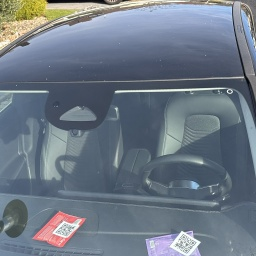
\includegraphics[width=0.3\textwidth]{Beispielpatch_0.jpg}
    \hfill
    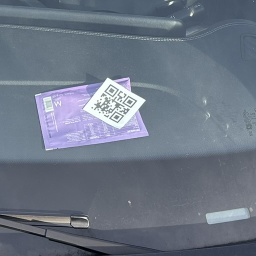
\includegraphics[width=0.3\textwidth]{Beispielpatch_2.jpg}
    \hfill
    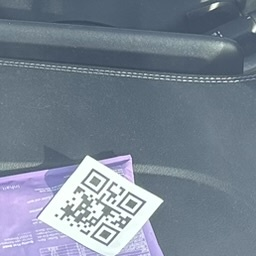
\includegraphics[width=0.3\textwidth]{Beispielpatch_4.jpg}
    
    \caption{Drei unterschiedliche SlidingWindow-Größen bei der gleichen Bildregion}
    \label{fig:patch_overlap}
\end{figure}

\subsection{Modelldurchlauf}

Nachdem das Bild durch das Sliding-Window-Verfahren in eine Menge normalisierter Patches zerlegt wurde, erfolgt der eigentliche Modelldurchlauf. In dieser Phase fungiert das neuronale Netz als Klassifikator, um für jeden einzelnen Bildausschnitt die Wahrscheinlichkeit zu bestimmen, mit der dieser einen QR-Code enthält.

\subsubsection{Datenvorbereitung und Farbraumanpassung}

Ein kritischer Schritt vor der eigentlichen Inferenz ist die Anpassung der Bilddaten an das gewählte Modell. Da die Inferenz-Pipeline flexibel verschiedene Architekturen unterstützt, findet eine dynamische Vorverarbeitung statt:
\begin{itemize}
    \item \textbf{Original-Modell:} Für das selbst entwickelte CNN-Modell werden die Patches in Graustufen geladen und um eine Kanaldimension erweitert, um dem erwarteten Eingangsformat zu entsprechen.
    \item \textbf{Transfer-Learning-Modelle:} Bei Modellen wie MobileNetV2 oder EfficientNetB0 erfolgt eine Konvertierung vom OpenCV-Standard BGR in den RGB-Farbraum. 
\end{itemize}
Zusätzlich werden alle Bilddaten in den Datentyp \texttt{float32} konvertiert, um eine präzise Verarbeitung durch die Gewichte des neuronalen Netzes zu gewährleisten.

\subsubsection{Batch-Verarbeitung und VRAM-Management}

Um die Inferenzzeit bei der hohen Anzahl an extrahierten Patches (oft mehrere hundert pro Bild) zu minimieren, werden diese gesammelt in Batches verarbeitet. Dies erlaubt es der Grafikhardware, die Berechnungen durch massive Parallelisierung zu beschleunigen. 

Da die Anzahl der Patches bei hochauflösenden 4K-Aufnahmen den verfügbaren Grafikspeicher (VRAM) überschreiten kann, wurde ein robustes Fehlermanagement implementiert. Das System nutzt eine iterative Batch-Größen-Anpassung: Sollte ein \texttt{ResourceExhaustedError} auftreten, wird die Batch-Größe halbiert und der Arbeitsspeicher bereinigt, bis die Inferenz stabil durchgeführt werden kann. Nach jedem Bilddurchlauf wird zudem die Keras-Session zurückgesetzt, um Speicherlecks langfristig zu vermeiden.

\begin{lstlisting}[language=Python, caption={Logik des Modelldurchlaufs mit dynamischem VRAM-Schutz}]
# Vorhersage mit dynamischer Batch-Groesse
preds = None
current_bs = cfg.start_batch_size
while current_bs >= 1:
    try:
        preds = model.predict(input_batch, batch_size=current_bs, verbose=0)
        break 
    except tf.errors.ResourceExhaustedError:
        print(f"VRAM Limit erreicht, reduziere Batch auf {current_bs // 2}")
        current_bs //= 2
        gc.collect()
\end{lstlisting}

\subsection{Heatmap Erstellung}

Das Ergebnis des Modelldurchlaufs ist eine Liste von Wahrscheinlichkeiten für alle extrahierten Patches. Da sich die Sliding Windows aufgrund des gewählten Overlaps und der verschiedenen Skalierungsstufen vielfach überschneiden, liegen für fast jede Bildregion mehrere Vorhersagen vor. Die Heatmap dient dazu, diese verstreuten Informationen zu fusionieren und eine räumliche Wahrscheinlichkeitsverteilung über das gesamte Originalbild zu legen.

\subsubsection{Das Voting-Prinzip der Wahrscheinlichkeits-Akkumulation}

Die Erstellung der Heatmap folgt einem akkumulativen \glqq Voting-Verfahren\grqq . Hierzu wird zunächst eine Matrix in der exakten Dimension des Originalbildes mit Nullwerten initialisiert. Das System iteriert anschließend durch alle Patches und deren zugehörige Modellvorhersagen.

Ein Patch gibt nur dann eine \glqq Stimme\grqq\ ab, wenn seine Konfidenz den Schwellenwert \texttt{min\_vote\_prob} überschreitet. Ist dies der Fall, wird die gesamte Wahrscheinlichkeit auf den entsprechenden Bereich der Heatmap-Matrix addiert. Pixel, die Teil eines QR-Codes sind, befinden sich durch den Multi-Scale-Ansatz in zahlreichen positiven Patches unterschiedlicher Größe. Durch die Addition dieser Werte entstehen in der Matrix lokale Maxima, sogenannte Hotspots. Zufällige Fehlklassifikationen (False Positives), die meist nur in einer einzigen Skalierung oder an einer spezifischen Position auftreten, erreichen dadurch niemals die notwendige kumulierte Summe, um als Detektion gewertet zu werden.

\begin{figure}[H]
    \centering
    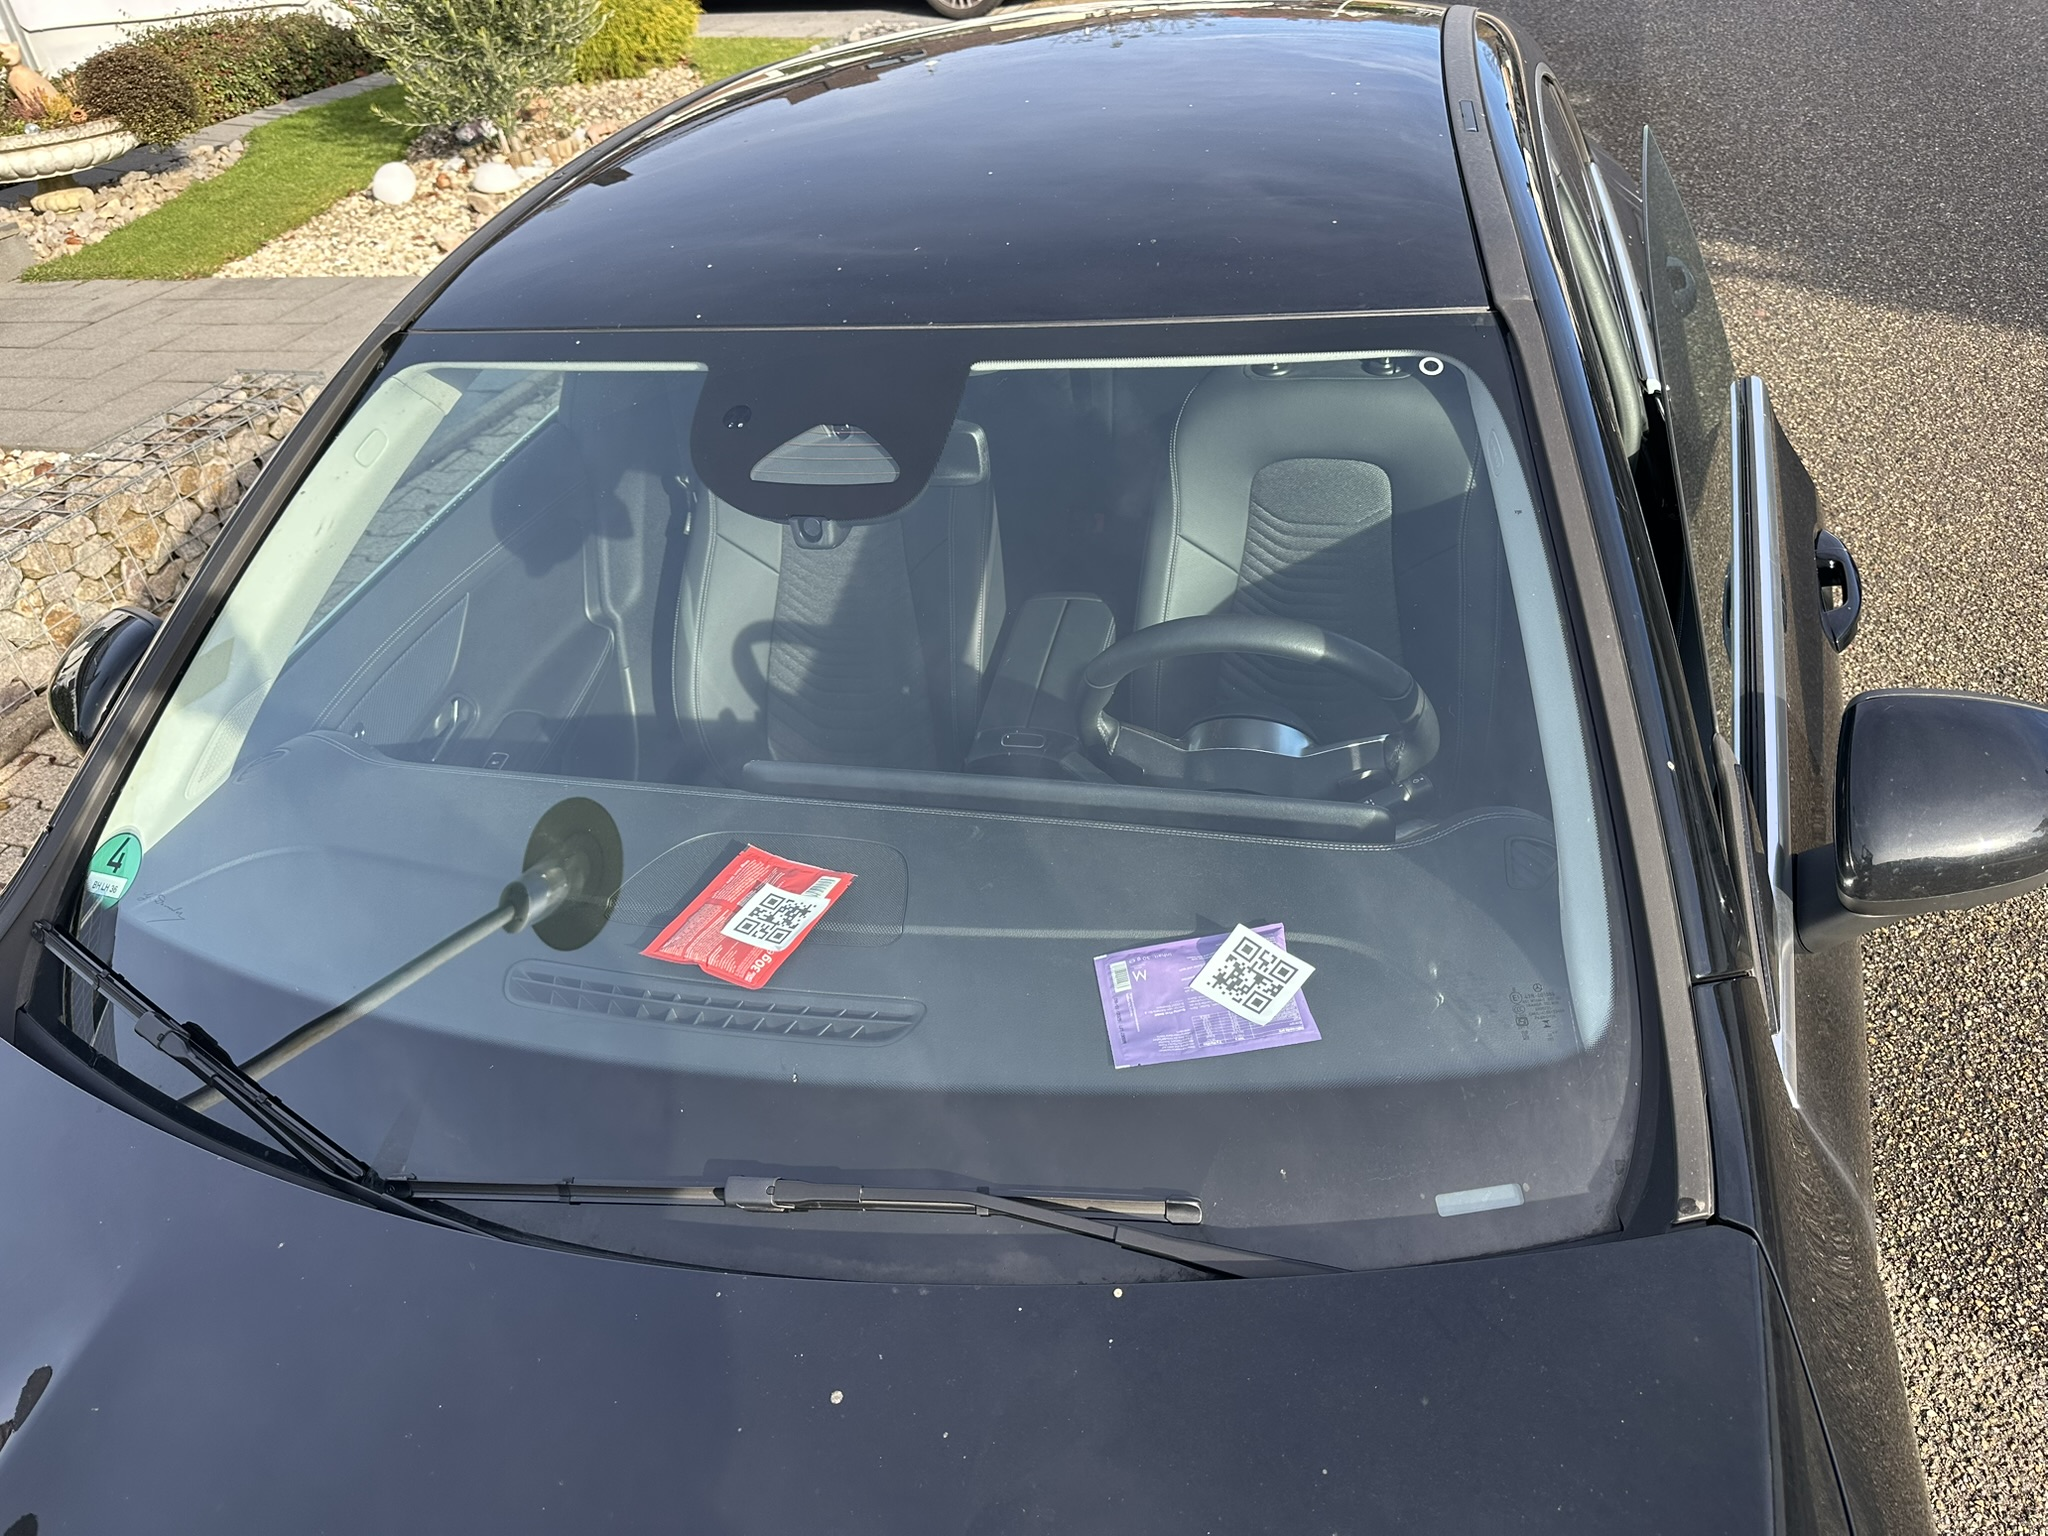
\includegraphics[width=0.47\textwidth]{Originalbild.png}
    \hfill
    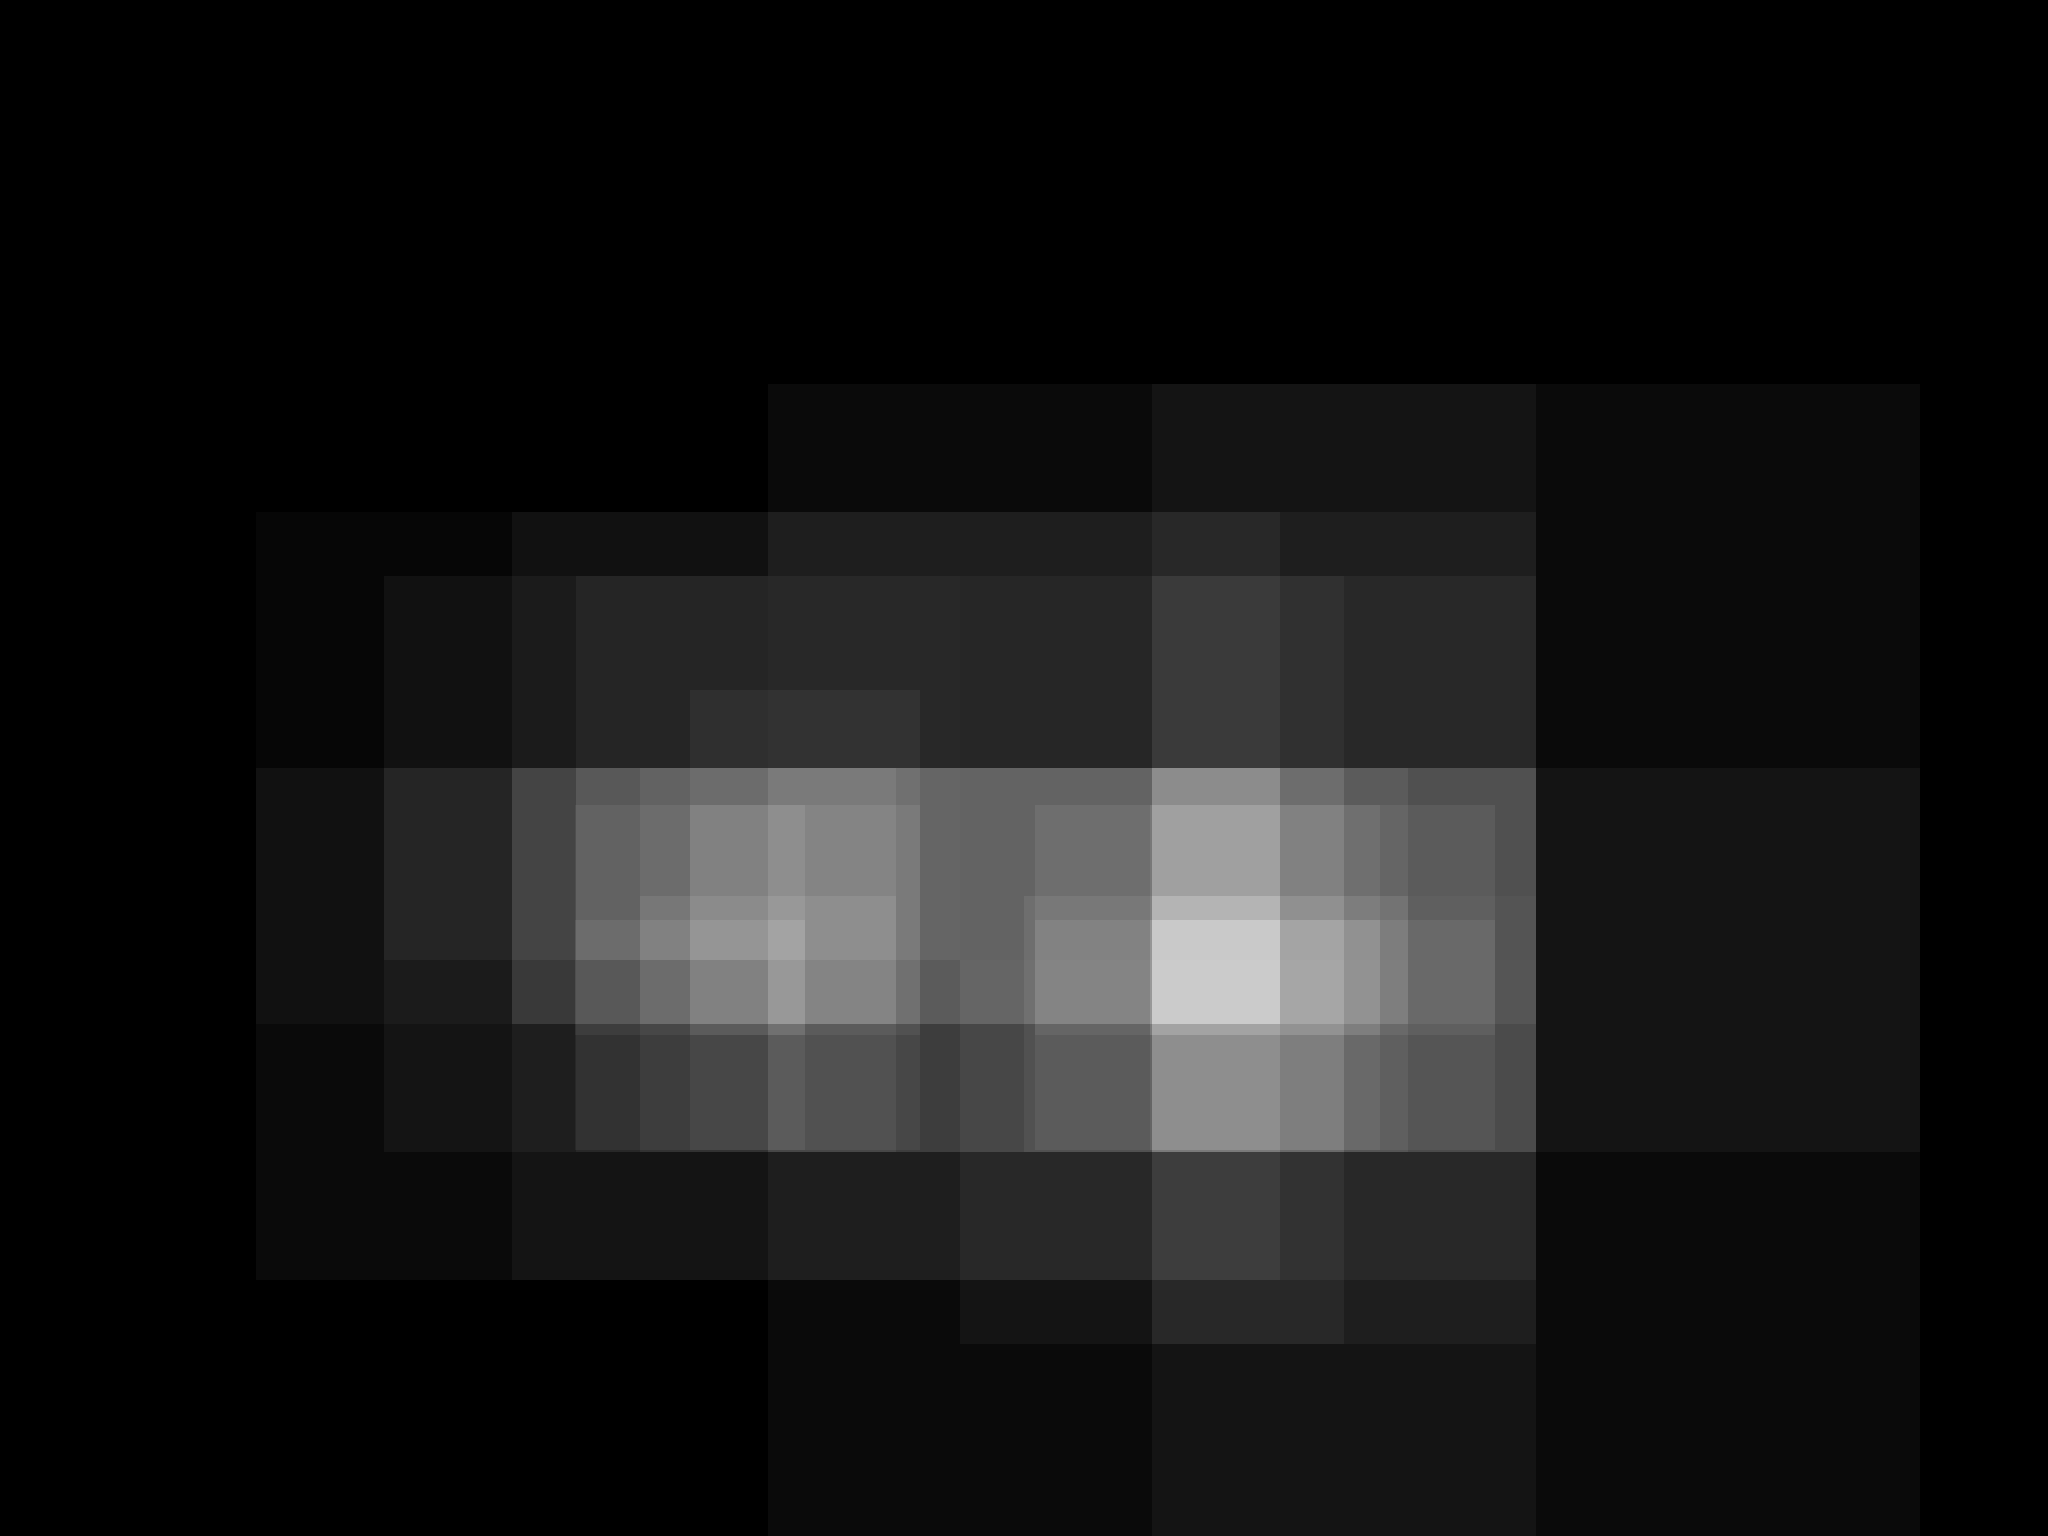
\includegraphics[width=0.47\textwidth]{Heatmap.png}
    \caption{Visualisierung des Prozesses: Vom Originalbild (links) zur akkumulierten Wahrscheinlichkeitsverteilung (rechts).}
    \label{fig:heatmap_process}
\end{figure}

\subsubsection{Konfigurationsparameter und Visualisierung}

Die Sensitivität und Präzision der Detektion lässt sich über drei zentrale Parameter steuern, die im Jupyter Notebook definiert sind:

\begin{table}[H]
    \centering
    \caption{Zentrale Parameter der Heatmap-Logik}
    \begin{tabular}{l p{9cm}}
        \toprule
        \textbf{Parameter} & \textbf{Bedeutung und Funktion} \\
        \midrule
        \texttt{min\_vote\_prob} & Ein Schwellenwert (z. B. 0.3), der als Filter fungiert. Nur Patches, die sich das Modell \glqq sicher genug\grqq\ ist, fließen in die Heatmap ein. \\
        \texttt{vote\_threshold} & Das finale Entscheidungskriterium (z. B. 5.0). Erst wenn die Summe der Wahrscheinlichkeiten an einer Stelle diesen Wert überschreitet, wird dort ein Objekt vermutet. \\
        \texttt{fixed\_vis\_max} & Dieser Parameter definiert den Endpunkt der Werteskala (z. B. 25.0) für die grafische Darstellung. Er legt fest, ab welcher Akkumulationsdichte ein Pixel in der Visualisierung als \glqq maximal heiß\grqq\ (weiß bzw. rot) dargestellt wird. \\
        \bottomrule
    \end{tabular}
\end{table}

\subsubsection{Visualisierung und Normierung (\texttt{fixed\_vis\_max})}

Da die aufsummierten Wahrscheinlichkeiten in der Heatmap-Matrix beliebige Werte annehmen können (z.\,B. eine Summe von 15,4), müssen diese für die Anzeige am Monitor in ein sichtbares Bild übersetzt werden. Ein digitaler Pixel kann Helligkeitswerte von 0 (Schwarz/Blau) bis 255 (Wei\ss/Rot) annehmen.

\begin{figure}[H]
    \centering
    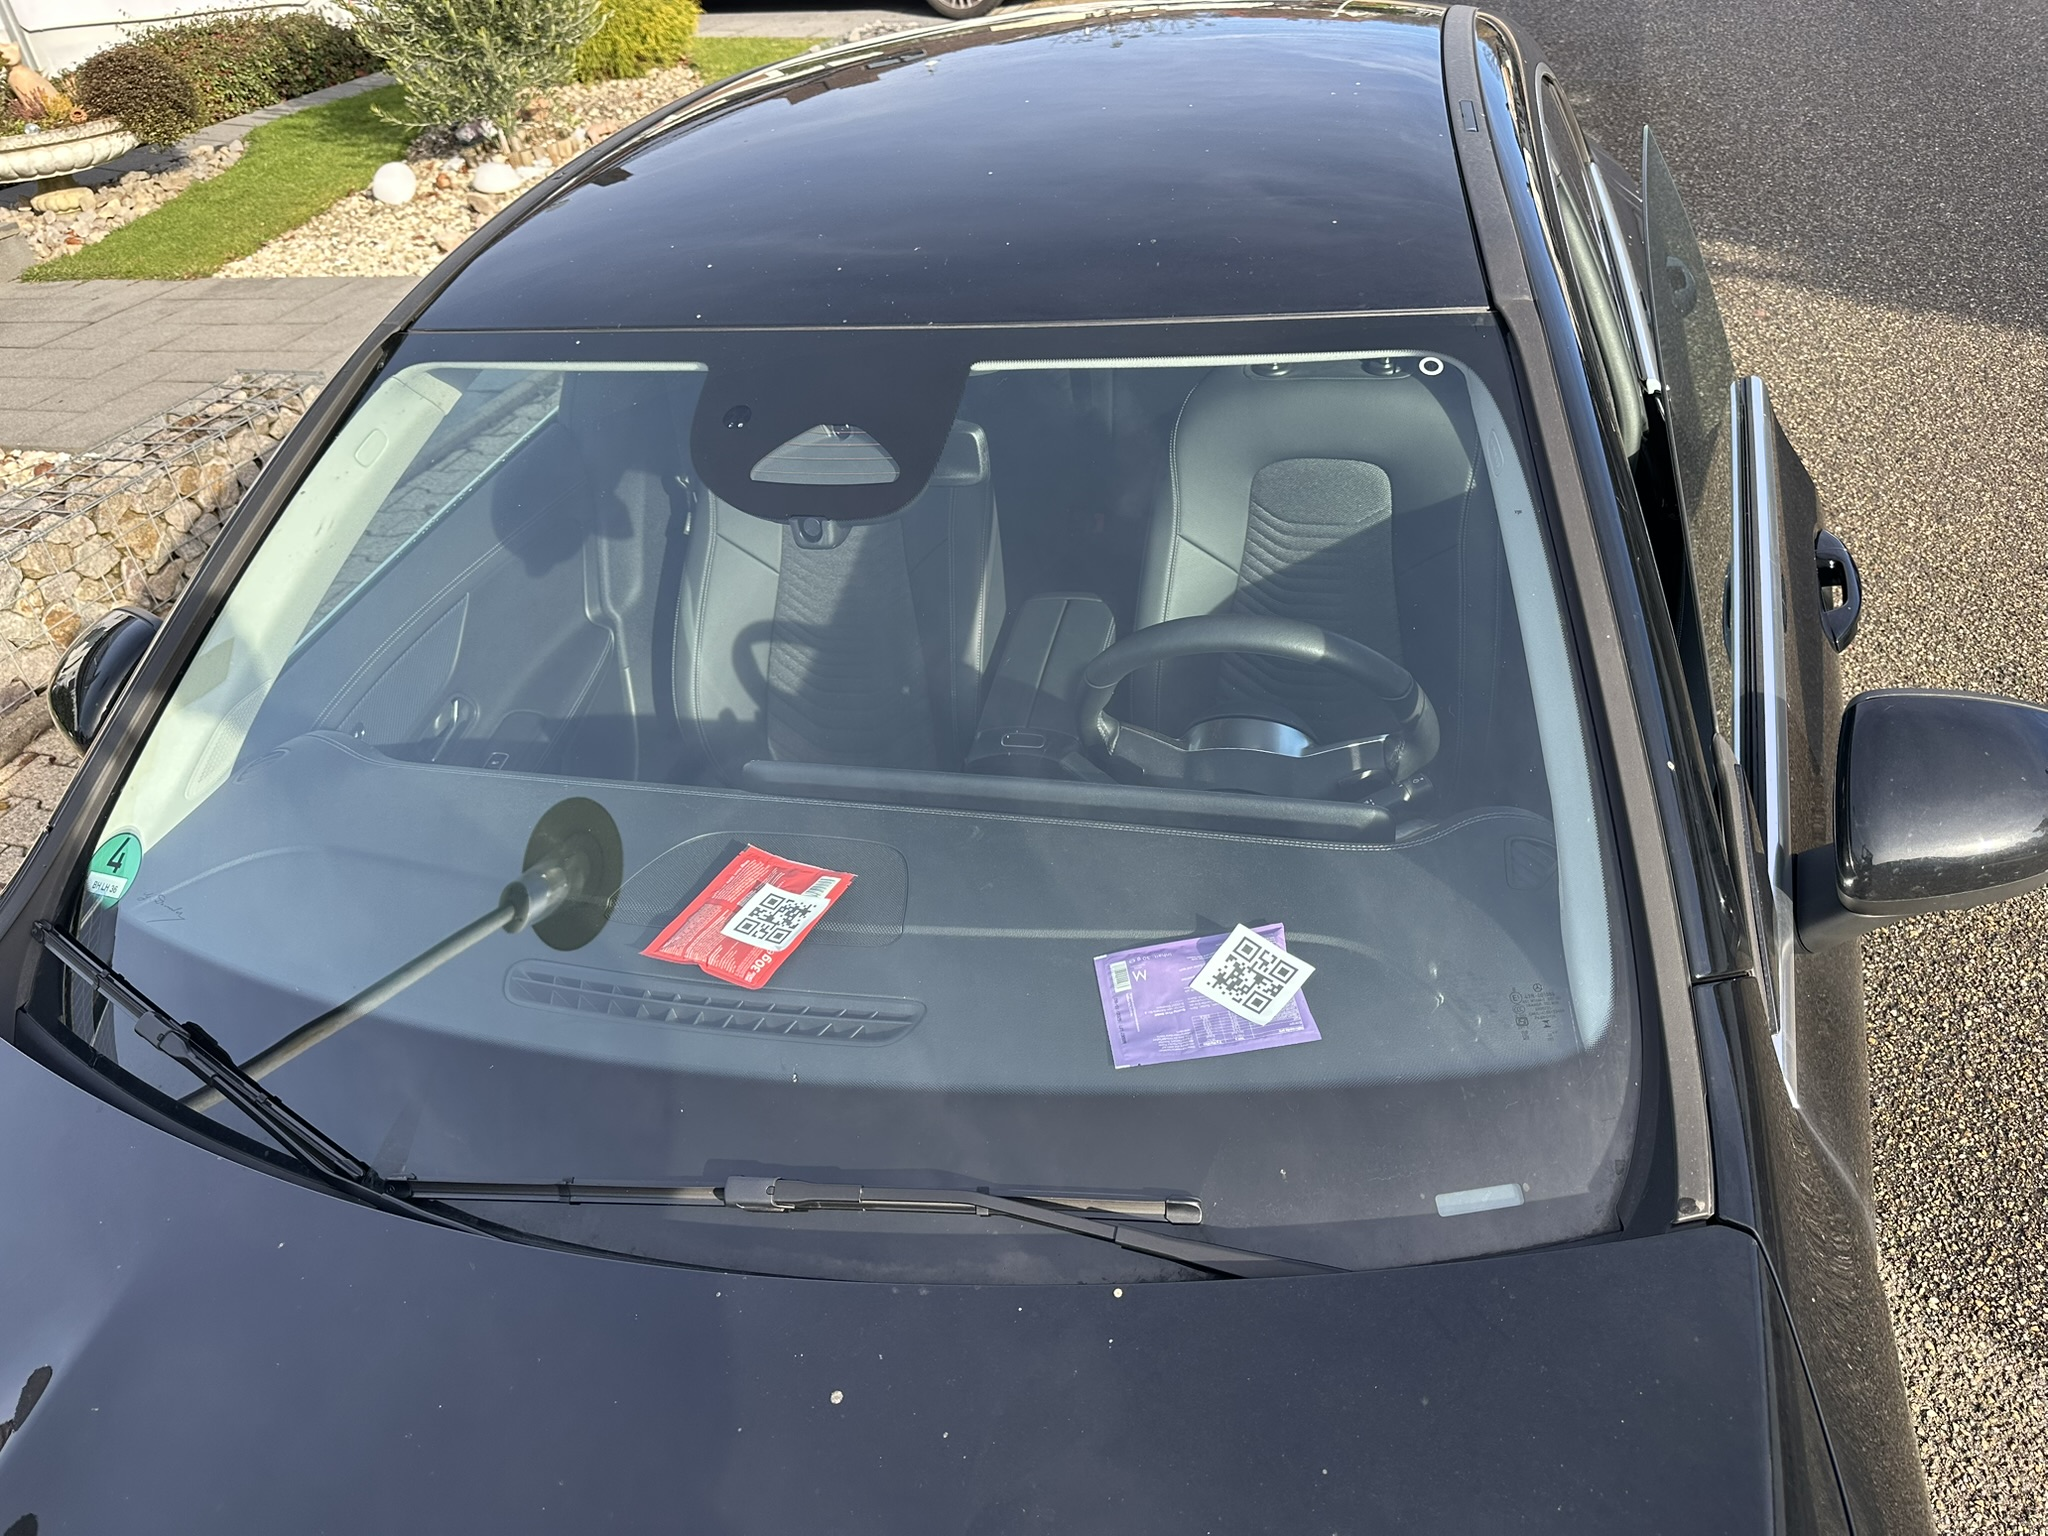
\includegraphics[width=0.47\textwidth]{Originalbild.png}
    \hfill
    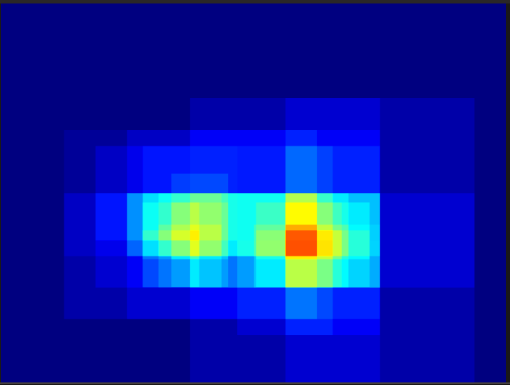
\includegraphics[width=0.47\textwidth]{Heatmap_bunt.png}
    \caption{Finale normierte Heatmap: Die roten Bereiche markieren die Zentren der detektierten QR-Codes mit höchster Konfidenz.}
    \label{fig:final_heatmap_example}
\end{figure}

Hierbei kommt der Parameter \texttt{fixed\_vis\_max} zum Einsatz. Er fungiert als \glqq Sättigungsgrenze\grqq\ bzw. als Messlatte für die maximale Helligkeit. Er definiert, ab welcher kumulierten Wahrscheinlichkeit ein Bereich im Bild als wei\ss\ / rot (maximal sicher) dargestellt werden soll. Die Umrechnung erfolgt nach der Formel:

$$\text{Pixelhelligkeit} = \min\left( \frac{\text{Akkumulierte Summe}}{\text{fixed\_vis\_max}} \cdot 255,\, 255 \right)$$

Durch diese Normierung werden die mathematischen Hotspots in eine für den Menschen interpretierbare Form übersetzt. Bereiche mit hoher Übereinstimmung erscheinen hell leuchtend, während unsichere Bereiche oder vereinzelte Fehlklassifikationen dunkel bleiben. Dies ermöglicht eine intuitive Beurteilung, wie sicher sich das System bei der Lokalisierung des QR-Codes ist.

\begin{figure}[H]
    \centering
    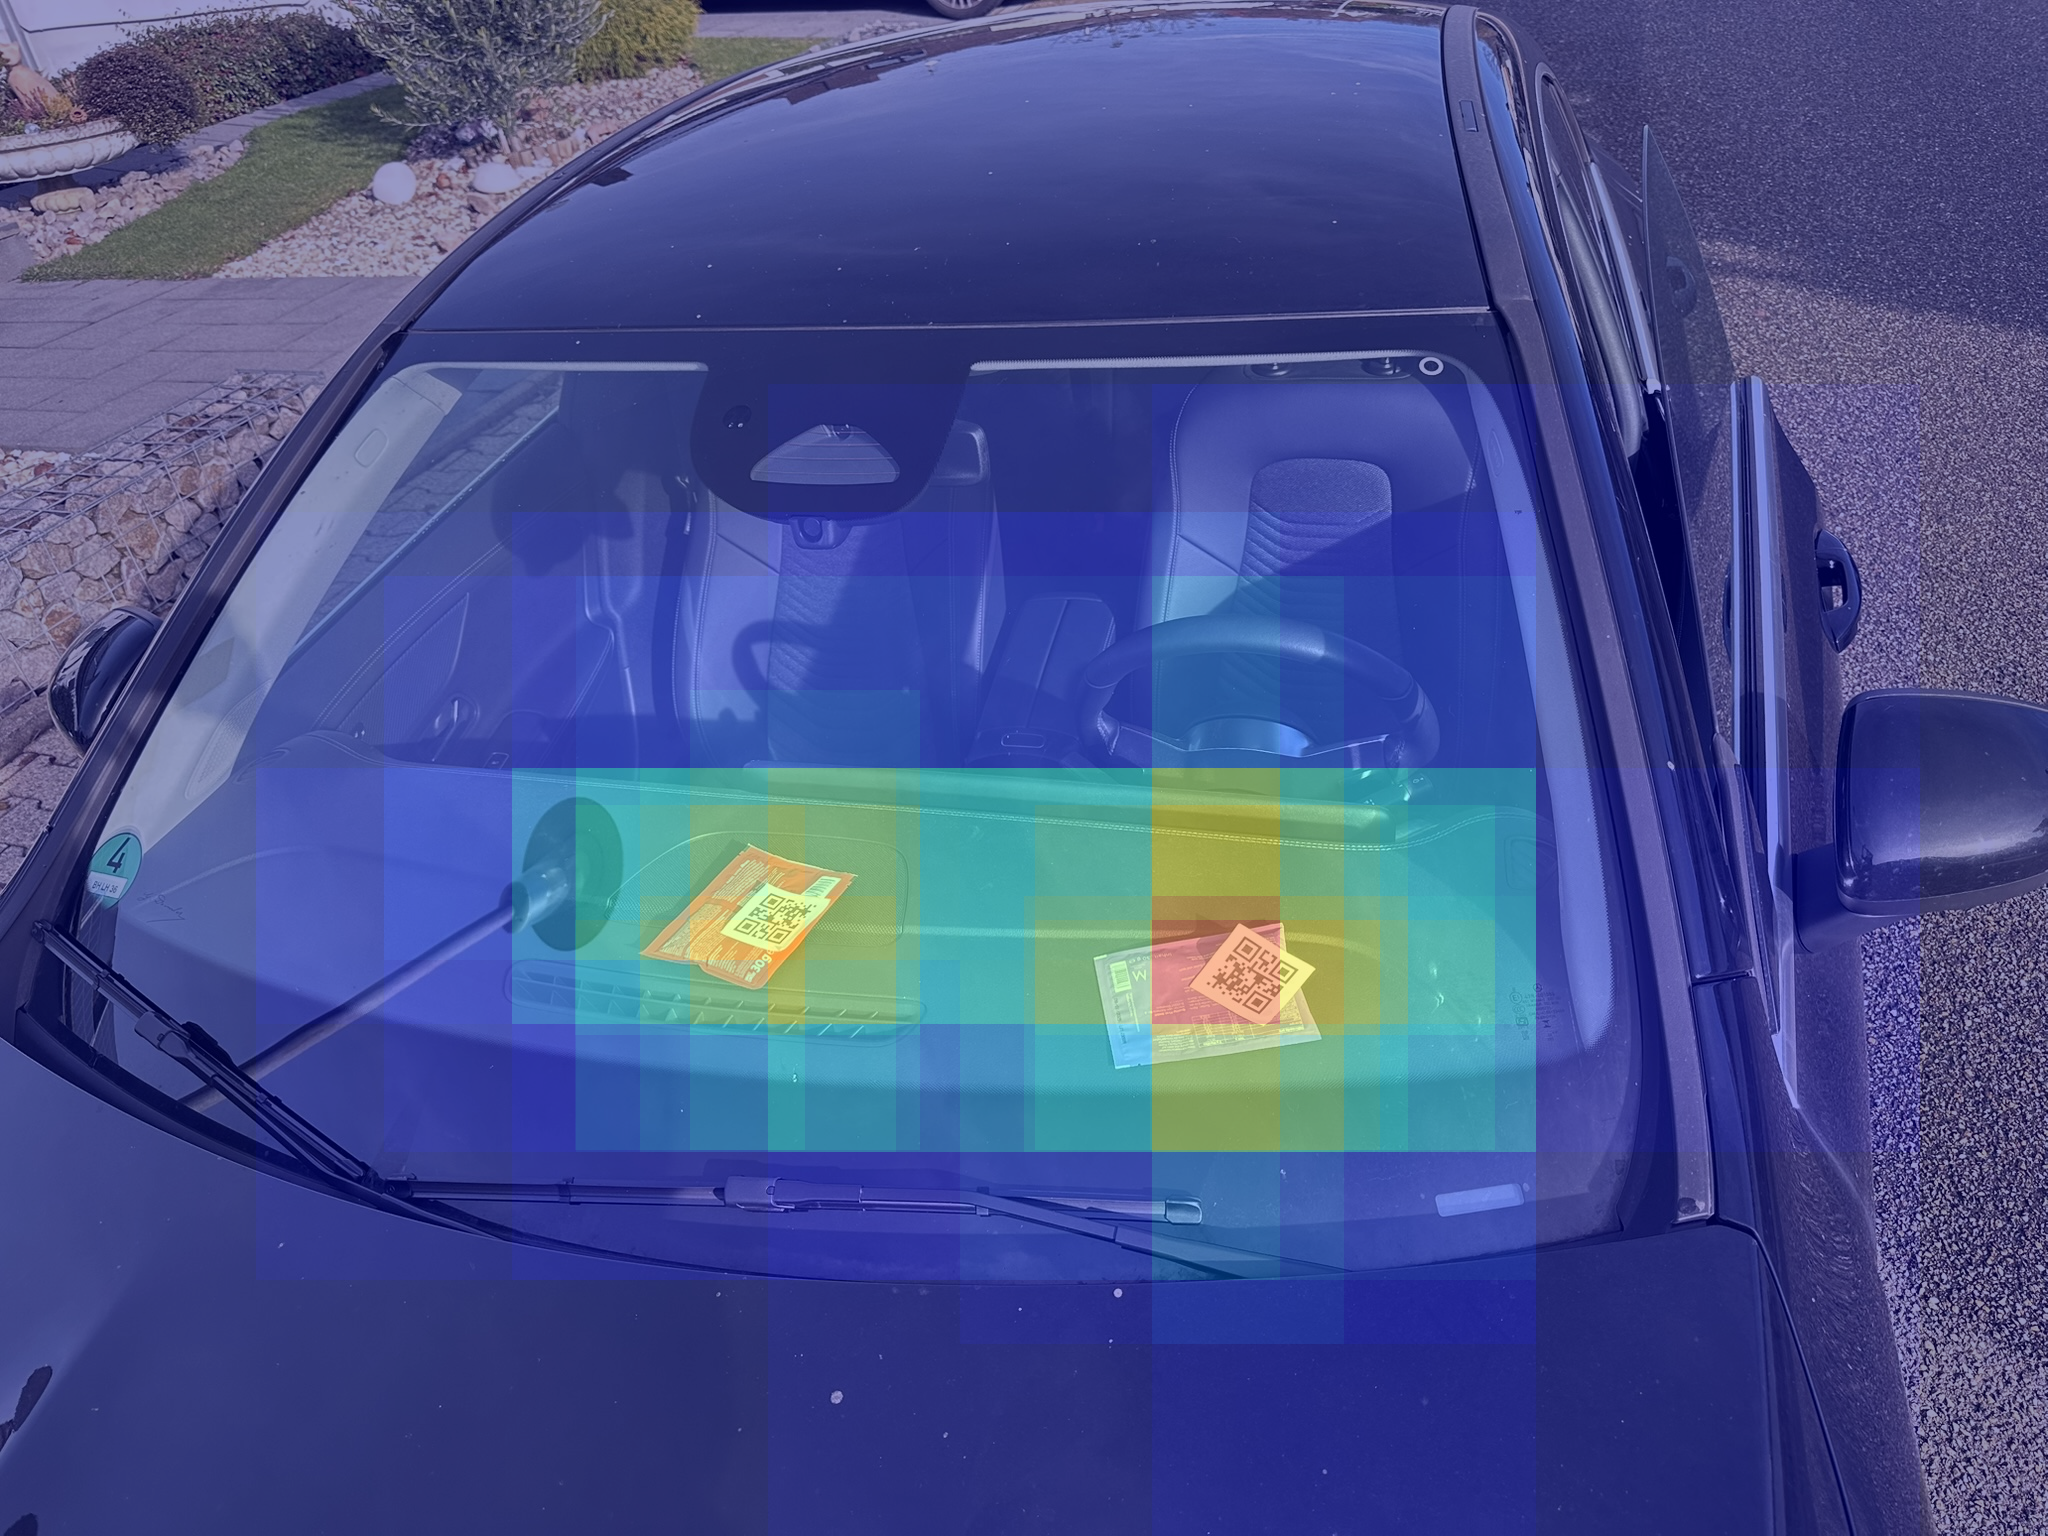
\includegraphics[width=0.5\textwidth]{Heatmap_auf_Orginalbild.png}
    \hfill
    \caption{Überlagerung der Heatmap auf das Originalbild}
    \label{fig:final_heatmap_example}
\end{figure}

\subsection{Finale Entscheidung und Lokalisierung}

Nach der Erstellung der Heatmap muss das System eine binäre Entscheidung treffen, ob ein QR-Code im Bild vorhanden ist. % 
In diesem abschließenden Schritt der Inferenz-Pipeline werden die kontinuierlichen Wahrscheinlichkeitswerte der Heatmap in präzise Koordinaten umgewandelt. % 

\subsubsection{Binarisierung: Trennung von Signal und Rauschen}

Die Heatmap lässt sich grafisch als eine Landschaft mit unterschiedlich hohen Erhebungen beschreiben, wobei die Höhe der \glqq Berge\grqq\ die Wahrscheinlichkeit für einen QR-Code repräsentiert. % 
Um daraus eine eindeutige Entscheidung abzuleiten, wird diese Landkarte in ein klares Schwarz-Wei\ss-Bild (Binärmaske) transformiert. % 

Hierbei fungiert der \texttt{vote\_threshold} als eine Art \glqq Türsteher\grqq: Nur Bereiche, die in der Summe genug Stimmen (z.\,B. einen kumulierten Wert von 5,0) gesammelt haben, werden als wei\ss\ markiert. % 
Alle Bereiche unterhalb dieses Wertes werden auf Null gesetzt und somit als Hintergrund (schwarz) eingestuft. % 
Dieser Schritt ist entscheidend für die Stabilität des Systems, da vereinzelte Fehlklassifikationen, die nur in einem einzelnen Patch auftraten, niemals die notwendige Stimmenanzahl erreichen und somit rigoros herausgefiltert werden. % 

\subsubsection{Lokalisierung und geometrische Plausibilitätsprüfung}

Nach der Bereinigung der Heatmap liegen oft isolierte wei\ss e Flächen vor, die potenzielle Standorte von QR-Codes markieren. % 
Um diese Flächen als eigenständige Objekte greifbar zu machen, wird ein Algorithmus zur Konturfindung (\texttt{cv2.findContours}) eingesetzt, der zusammenhängende Pixel-Inseln identifiziert und deren Au\ss engrenzen definiert. % 



Jede gefundene Kontur wird anschließend einer geometrischen Plausibilitätsprüfung unterzogen, um Fehlalarme durch optisches Rauschen oder feine Hintergrundmuster auszuschlie\ss en. % 
Hierzu wird mit \texttt{cv2.boundingRect} das kleinste umschlie\ss ende Rechteck für jede Insel berechnet: % 
\begin{itemize}
    \item Da ein echter QR-Code im Kamerabild immer eine gewisse Mindestgröße aufweisen muss, werden extrem kleine Konturen (unter $30 \times 30$ Pixeln) ignoriert. % 
    \item Diese Filterung stellt sicher, dass nur signifikante Merkmale zur weiteren Analyse an den Decoder übergeben werden. % 
\end{itemize}

\subsubsection{Visualisierung der Detektion}

Wurde mindestens eine valide Kontur gefunden, gilt das Bild als \glqq QR DETECTED\grqq. Zur Dokumentation und visuellen Verifikation wird die Lokalisierung im Ausgabebild hervorgehoben:
\begin{itemize}
    \item \textbf{Bounding Box:} Um das detektierte Objekt wird ein grüner Rahmen mit einer definierten Linienstärke gezeichnet.
    \item \textbf{Status-Anzeige:} Im Evaluation-Dashboard wird zusätzlich der berechnete \glqq Real Score\grqq\ (die maximale Dichte der Heatmap) sowie die finale Entscheidung ausgegeben.
\end{itemize}

\begin{figure}[H]
    \centering
    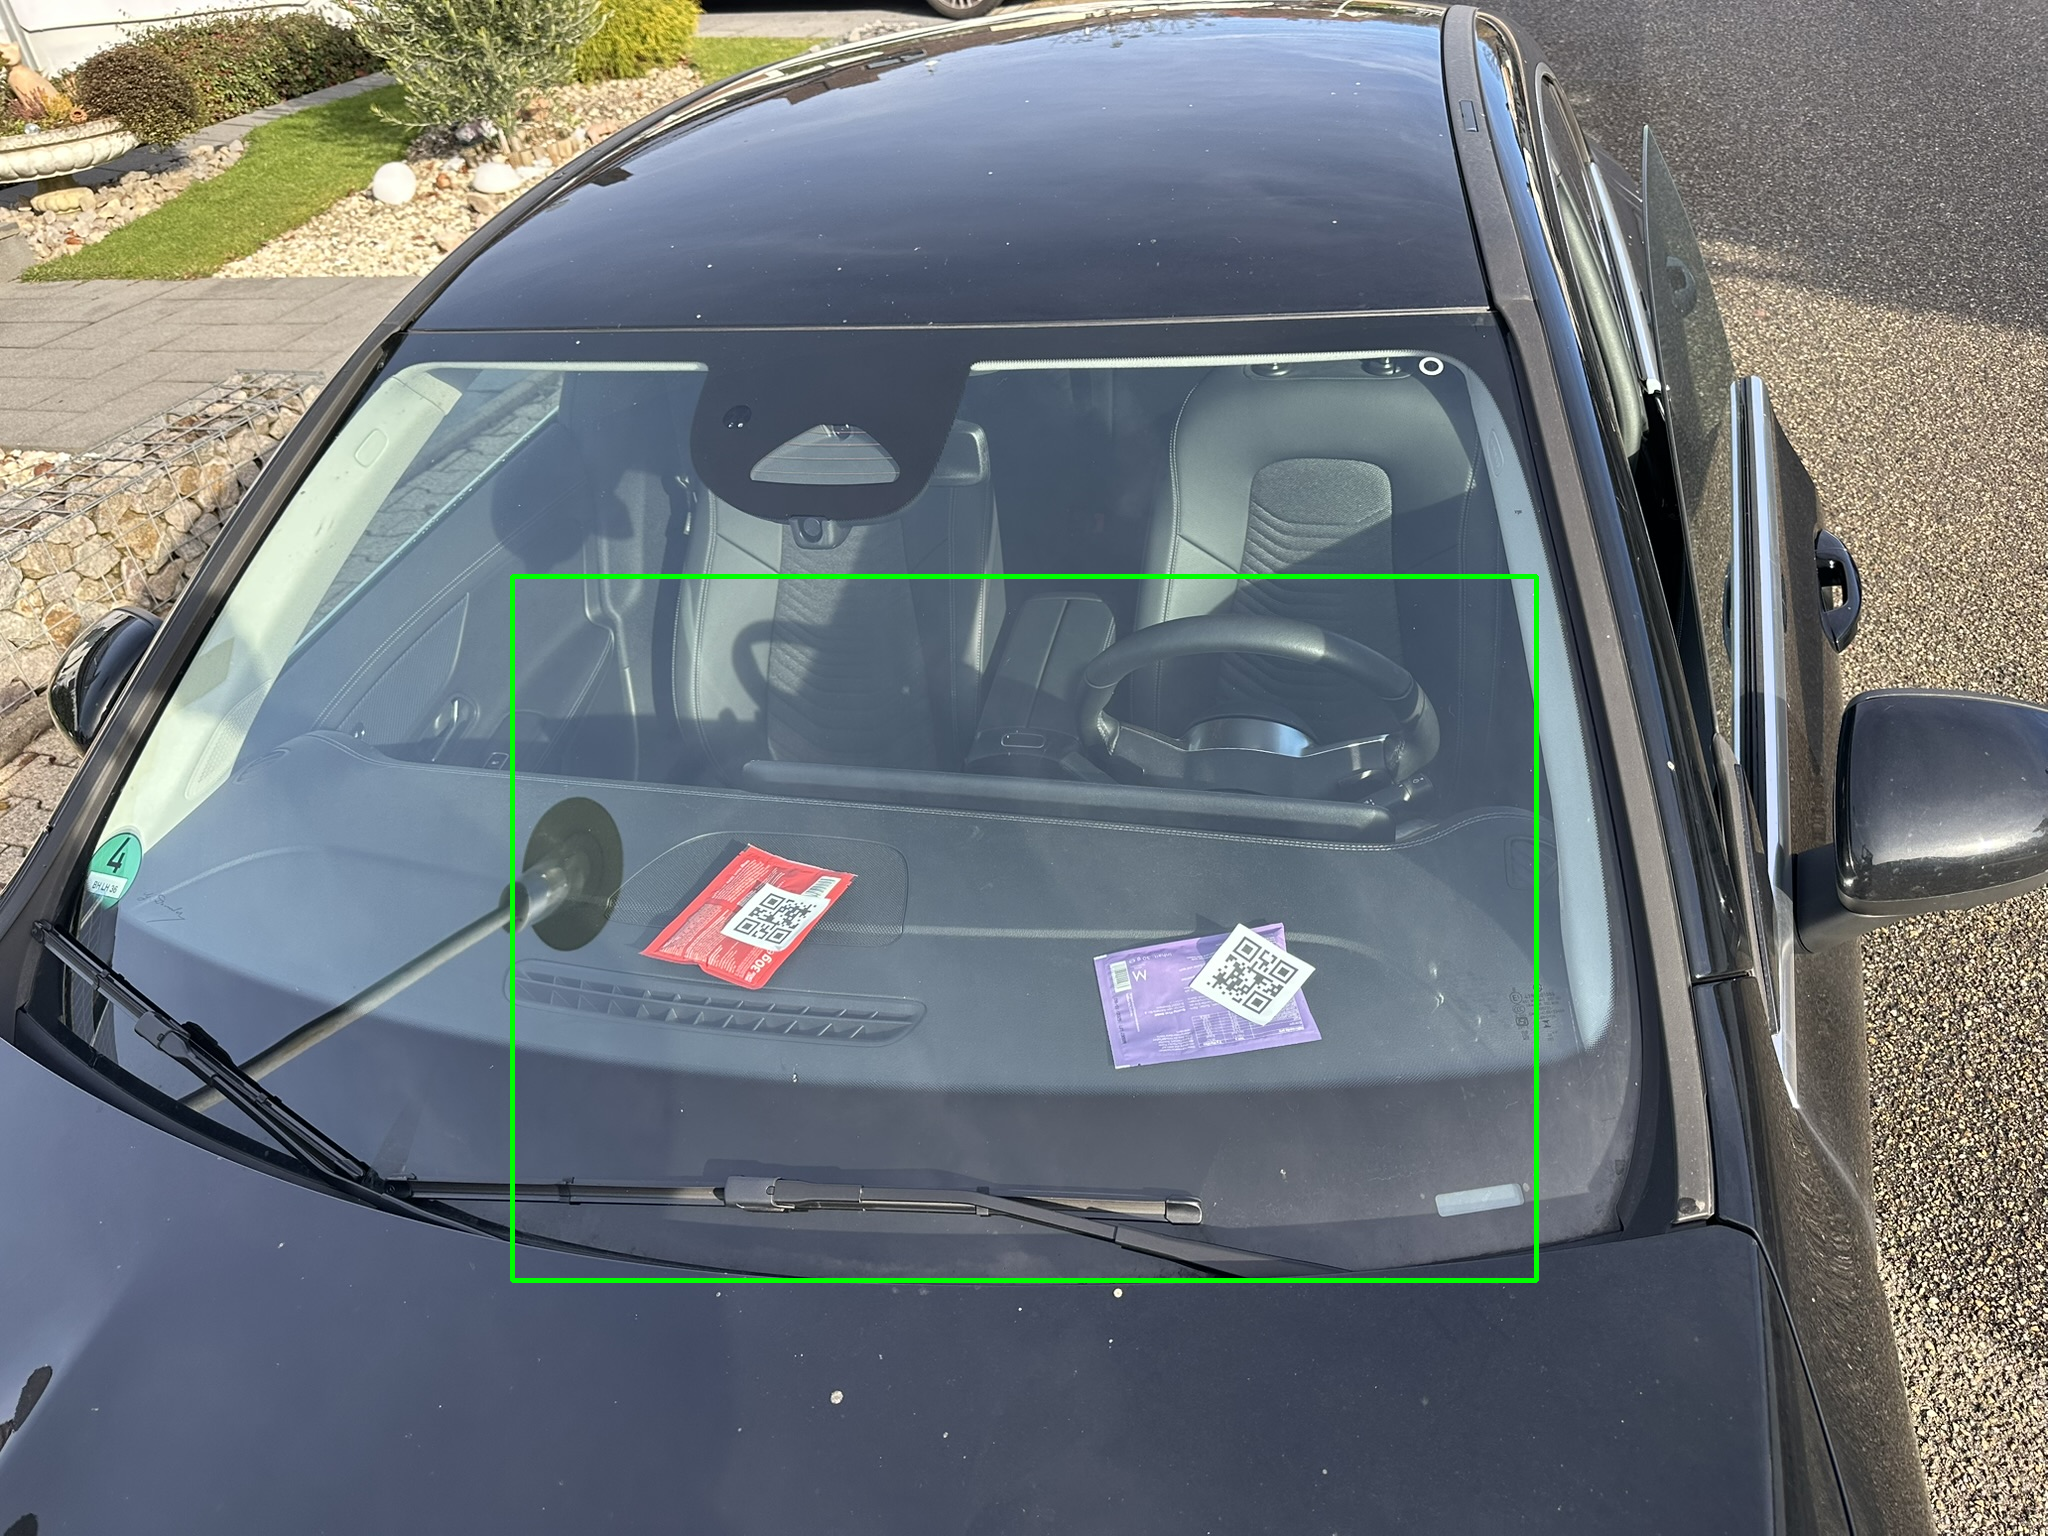
\includegraphics[width=0.8\textwidth]{ROI_Kennzeichnung.PNG}
    \caption{Finales Ergebnis der Inferenz: Der lokalisierte QR-Code wird durch eine grüne Bounding Box im Originalbild hervorgehoben.}
    \label{fig:final_decision}
\end{figure}

Sollten keine Konturen den \texttt{vote\_threshold} und die Größenfilterung passieren, wird das Bild als \glqq NO DETECTION\grqq\ markiert. Dies stellt sicher, dass die nachgelagerte und rechenintensive Decodierung nur auf Bildbereichen ausgeführt wird, in denen mit hoher Sicherheit ein QR-Code vorliegt.

\subsubsection{Visuelle Ergebniskontrolle: Das Evaluations-Dashboard}

Das zur Ergebniskontrolle implementierte Dashboard führt die Ergebnisse der Inferenz-Pipeline in einer kompakten $2 \times 2$-Ansicht zusammen. Anstatt die Teilschritte isoliert zu betrachten, ermöglicht die simultane Gegenüberstellung von Originalbild, Heatmap, Overlay und finaler ROI-Kennzeichnung einen unmittelbaren Abgleich zwischen der internen Wahrscheinlichkeitsverteilung und dem physischen Bildinhalt.

Ergänzend zur grafischen Übersicht liefert die Statuszeile im Footer die Fakten für die weitere Prozesssteuerung: Hier werden der \texttt{max\_score} als numerischer Beleg für die Detektionssicherheit sowie die finale Systementscheidung (\glqq QR DETECTED\grqq\ oder \glqq NO DETECTION\grqq) ausgegeben. Diese Zusammenfassung markiert den Abschluss der Detektionsphase und die Freigabe der identifizierten Bildbereiche für die nachgelagerte Dekodierung.

\begin{figure}[H]
    \centering
    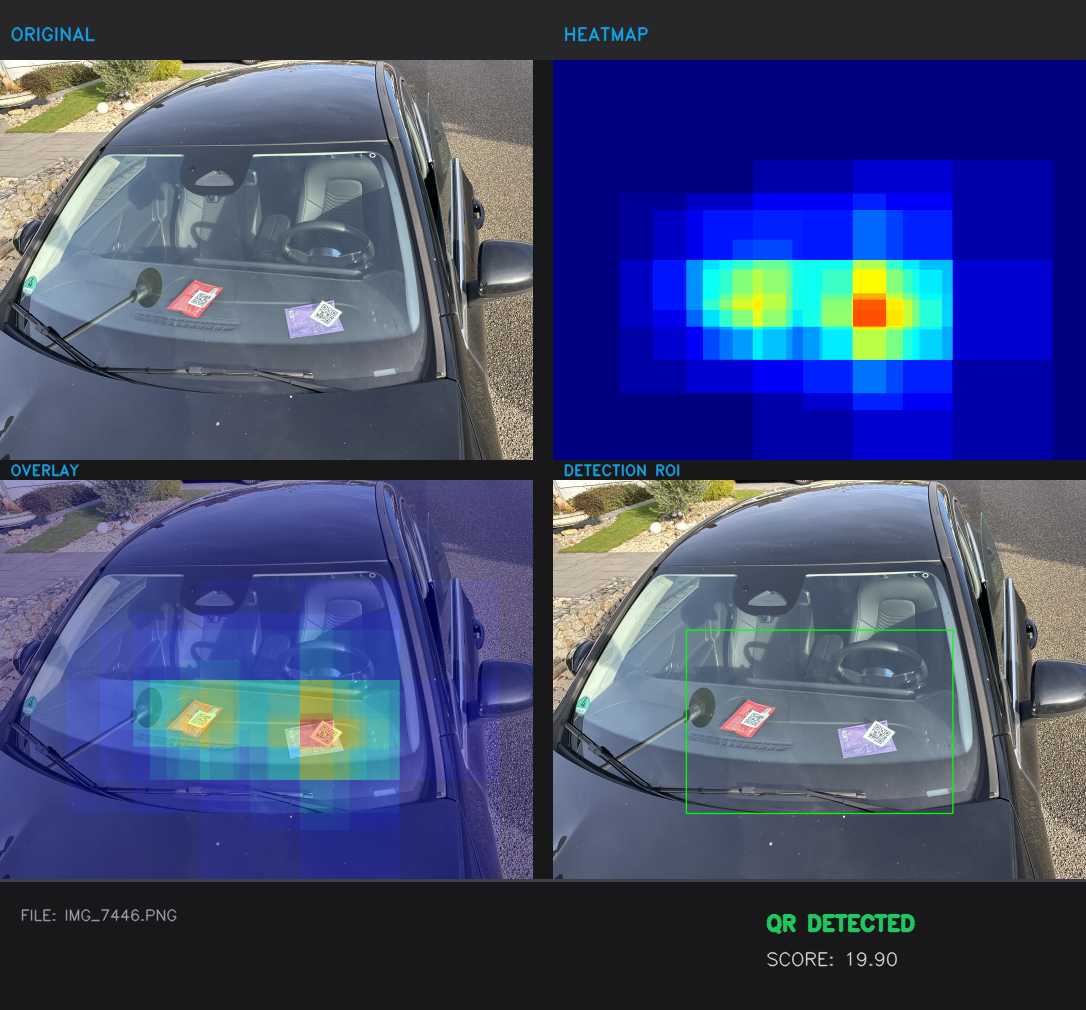
\includegraphics[width=0.8\textwidth]{GUI.png}
    \caption{Dashboardübersicht QR DETECTED.}
    \label{fig:final_decision}
\end{figure}

\begin{figure}[H]
    \centering
    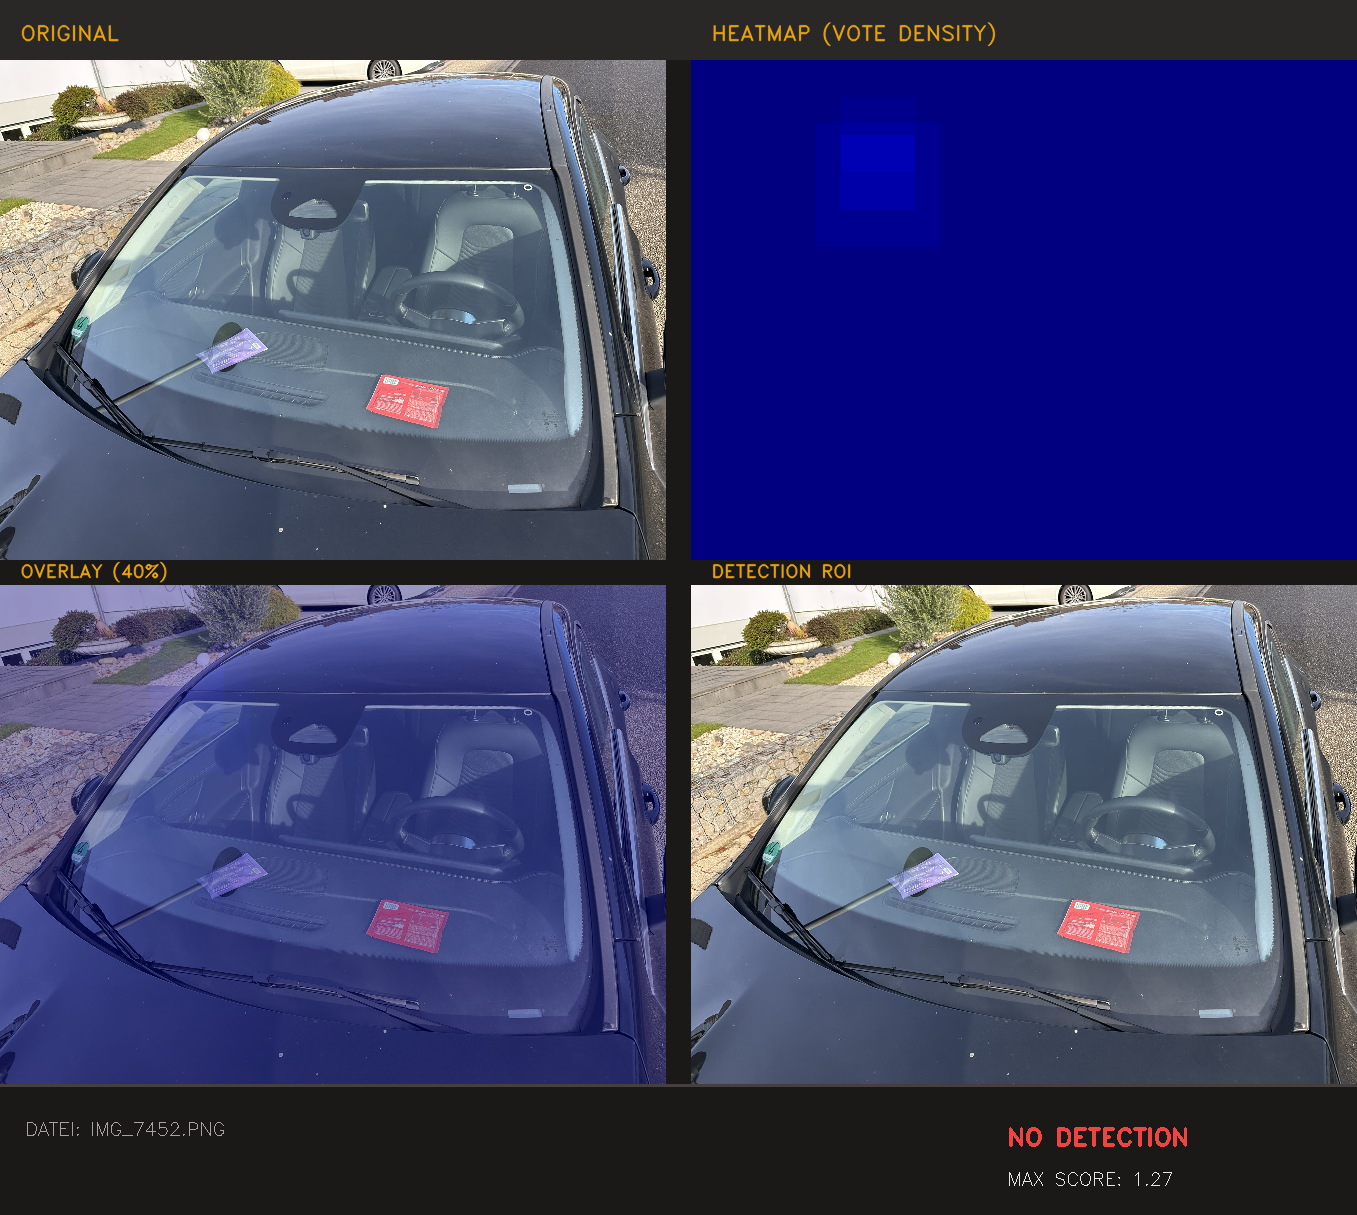
\includegraphics[width=0.8\textwidth]{GUI_negativ.png}
    \caption{Dashboardübersicht NO DETECTION.}
    \label{fig:final_decision}
\end{figure}

% ==========================================
% KAPITEL 6: ENTSCHLÜSSELUNG DER QR-CODES
% ==========================================
\section{Entschlüsselung der QR-Codes}

Nachdem die Inferenzphase potenzielle Regionen (ROIs) identifiziert hat, folgt der entscheidende Schritt der Inhaltsanalyse. Ziel ist es, die grafischen Bit-Muster in einen digitalen Datenstring zu überführen. Da die Bildaufnahme unter realen Bedingungen einer Waschanlage erfolgt, muss das System eine hohe Resilienz gegenüber physikalischen Störeinflüssen aufweisen.

\subsection{Aufgabe und Herausforderungen}
Die Schwierigkeit der Extraktion liegt in der massiven Abweichung von einer idealen Scan-Geometrie. Während kommerzielle Handscanner eine frontale, planparallele Ausrichtung erwarten, agiert dieses System unter erschwerten Bedingungen:
\begin{itemize}
    \item \textbf{Perspektivische Distorsion:} Durch den steilen Aufnahmewinkel der Kamera zur Windschutzscheibe wird das Quadrat des Codes zu einem Trapez verzerrt. Dies verschiebt die Position der Datenbits relativ zu den Synchronisationsmustern.
    \item \textbf{Optische Diffraktion:} Wassertropfen auf der Scheibe wirken wie Mikrolinsen, die lokale Kontraste invertieren oder Kanten verschwimmen lassen.
    \item \textbf{Dynamische Reflexionen:} Lichtbrechungen auf der Glasoberfläche überlagern die Bit-Matrix mit Störsignalen, die für klassische Decoder wie Rauschen wirken.
\end{itemize}


\subsection{Methodik: Detaillierte Analyse der Dekodierungsansätze}
Um eine möglichst robuste Erkennung zu gewährleisten, wurden drei technologisch unterschiedliche Strategien entwickelt und an einem umfangreichen Test-Datensatz von insgesamt 4.128 Bildern evaluiert. Davon enthielten 3.111 Bilder einen relevanten QR-Code unter Realbedingungen (Nässe, Schaum, extreme Winkel). Die Ansätze verfolgen grundlegend verschiedene Philosophien: von der klassischen Bildverbesserung über statistische Aufteilung bis hin zu moderner künstlicher Intelligenz.

\subsubsection{Ansatz 1: Pixel-basierte Bildrestaurierung (Robust Restored)}
Dieser Ansatz folgt dem Prinzip der klassischen digitalen Bildbearbeitung. Die Kernannahme ist, dass ein QR-Code primär deshalb nicht gelesen werden kann, weil das Bild zu unscharf, zu kontrastarm oder durch Umwelteinflüsse wie beispielsweise einen leichten Wasserfilm \glqq verwaschen\grqq\ ist. Man kann sich diesen Ansatz wie eine automatische \glqq digitale Brille\grqq\ vorstellen, die versucht, das Bild für den Standard-Scanner zu optimieren.

Schlägt der erste Leseversuch auf dem Originalbild fehl, wird eine Kette von mathematischen Filtern aktiviert, um die Kanten des QR-Codes für den Computer deutlicher hervorzuheben:
\begin{itemize}
    \item \textbf{Detail-Verstärkung (Guided Filtering):} Hierbei wird das Bild in seine Grundstrukturen und seine feinen Details zerlegt. Die feinen Details – also die Kanten der QR-Code-Module – werden gezielt verstärkt, während großflächiges Rauschen unterdrückt wird.
    \item \textbf{Kanten-Schärfung (Laplace-Operator):} Ein mathematischer Filter sucht nach abrupten Helligkeitsübergängen (Schwarz-Weiß-Wechsel) und steilt diese extrem nach. Dies soll verhindern, dass der Scanner die einzelnen Punkte des Codes als grauen Brei wahrnimmt.
\end{itemize}

\begin{lstlisting}[language=Python, caption={Iterative Bildverbesserungskette in Ansatz 1}]
def run_decoding_restored(roi):
    # 1. Versuch: Dekodierung des Rohbildes
    result = decode(roi)
    if result: return result
    
    # 2. Versuch: Kantenanhebung (Detail Enhancement)
    # Ziel: Strukturen klarer vom Hintergrund abheben
    enhanced = cv2.detailEnhance(roi, sigma_s=10, sigma_r=0.15)
    result = decode(enhanced)
    if result: return result
    
    # 3. Versuch: Schaerfungs-Kernel zur Kontrastmaximierung
    kernel = np.array([[-1,-1,-1], [-1,9,-1], [-1,-1,-1]])
    sharpened = cv2.filter2D(roi, -1, kernel)
    return decode(sharpened)
\end{lstlisting}

\textbf{Evaluation:} Trotz der optischen Aufwertung erzielte dieser Ansatz lediglich eine Erfolgsquote von 22,3\,\%. Das Hauptproblem bleibt die Geometrie: Da die Filter zwar die Pixel deutlicher machen, aber die perspektivische Verzerrung (das Trapez) nicht korrigieren, erwartet der Standard-Scanner die Datenpunkte immer noch an der falschen Stelle.

\subsubsection{Ansatz 2: Räumliche Redundanz (Smart Tiling)}
Dieser Ansatz nutzt eine Eigenschaft von QR-Codes aus: ihre eingebaute Fehlertoleranz. Ein QR-Code muss nicht zu 100\,\% perfekt sichtbar sein, um gelesen zu werden; oft reichen schon 70\,\% der Fläche aus, um den Rest mathematisch zu ergänzen.

Die Idee von Divide-and-Conquer\grqq-Verfahren (Teile und Herrsche). Anstatt das gesamte, eventuell teilweise durch Schaum oder Reflexionen gestörte Bild zu scannen, wird die Region in fünf kleinere, überlappende Sektoren zerlegt: das Zentrum sowie die vier Ecken.
Die Logik dahinter: Wenn beispielsweise in der oberen linken Ecke ein dicker Wassertropfen das Bild verzerrt, ist das Zentrum oder die untere rechte Ecke vielleicht noch klar genug. Durch das separate Scannen dieser Teilbereiche erhöht man die statistische Chance, dass der Scanner in einem der Ausschnitte genügend saubere Daten findet, um den gesamten Inhalt zu rekonstruieren.

\begin{lstlisting}[language=Python, caption={Sektorale Aufteilung der ROI (Smart Tiling)}]
def combined_force_decode(roi):
    h, w = roi.shape[:2]
    # Aufteilung in 5 strategische Bereiche
    sectors = {
        "Center": roi[int(h*0.2):int(h*0.8), int(w*0.2):int(w*0.8)],
        "Top-Left": roi[0:int(h*0.7), 0:int(w*0.7)],
        "Top-Right": roi[0:int(h*0.7), int(w*0.3):w],
        "Bottom-Left": roi[int(h*0.3):h, 0:int(w*0.7)],
        "Bottom-Right": roi[int(h*0.3):h, int(w*0.3):w]
    }
    for name, patch in sectors.items():
        if res := robust_decode_func(patch):
            return res, name 
    return None, None
\end{lstlisting}

\textbf{Evaluation:} In der Praxis erwies sich dieser Ansatz als enttäuschend. Die Laufzeit vervielfachte sich, da pro Bild bis zu sechs Dekodierversuche unternommen wurden. Da die grundlegende perspektivische Verzerrung auch in den kleinen Ausschnitten bestehen bleibt, lag die Erfolgsquote kaum über der von Ansatz 1. 

\subsubsection{Ansatz 3: KI-basierte Detektion und Rektifizierung (QReader)}
Der dritte Ansatz unterscheidet sich fundamental von den vorherigen, da er das Problem nicht durch Bildfilter, sondern durch geometrisches Verständnis löst. Hierbei kommt die spezialisierte KI-Bibliothek \texttt{QReader} zum Einsatz.

Dieser Prozess läuft in zwei hochintelligenten Phasen ab:
\begin{enumerate}
    \item \textbf{KI-Suche (YOLOv8):} Ein neuronales Netz, das speziell darauf trainiert wurde, QR-Codes auch unter extremen Winkeln und bei schlechter Sicht zu finden, scannt den Bildbereich. Dabei ist die Empfindlichkeit sehr hoch eingestellt, sodass auch stark verzerrte Codes erkannt werden.
    \item \textbf{Digitale Rektifizierung (\glqq Bügeln\grqq):} Das ist der entscheidende Schritt. Die KI erkennt die vier exakten Eckpunkte des QR-Codes, egal wie schief er im Bild liegt. Mithilfe einer mathematischen Transformation wird der verzerrte Code \glqq geradegezogen\grqq. Er wird virtuell so umgerechnet, als ob die Kamera frontal und perfekt plan davor stünde. Erst dieser perfekt quadratische Ausschnitt wird an den Scanner übergeben.
\end{enumerate}

\begin{lstlisting}[language=Python, caption={KI-gestuetzte Polygon-Extraktion mittels QReader}]
from qreader import QReader
reader = QReader(model_size='s') # Nutzt ein kompaktes YOLOv8-Modell

# Schritt 1: Finden der 4 Eckpunkte (Polygon)
detections = reader.detect(image=roi_rgb) 

for det in detections:
    # Schritt 2: Mathematische Entzerrung und Auslesen
    content = reader.decode(image=roi_rgb, detection_result=det)
    if content:
        # Die Eckpunkte werden fuer die Winkelberechnung gespeichert
        poly_points = det['polygon_xy'] 
\end{lstlisting}

\textbf{Evaluation:} Mit einer Erfolgsquote von 33,9\,\% ist dies der mit Abstand leistungsfähigste Ansatz. Er ist der einzige, der die physikalischen Realitäten einer schrägen Windschutzscheibe wirklich kompensieren kann.

\subsection{Finale Entscheidung}
Die abschließende Evaluation führt zu einer eindeutigen Entscheidung für den \textbf{KI-basierten Ansatz mittels QReader}. Mehrere Faktoren gaben hierfür den Ausschlag:

Erstens ist die \textbf{Robustheit} unerreicht. Während klassische Methoden bei 22,3\,\% stagnieren, ermöglicht die KI-gestützte Rektifizierung eine signifikante Steigerung der Erkennungsrate. Dies ist besonders kritisch, da in einer Waschanlage die zuverlässige Identifikation auch unter schwierigsten Sichtbedingungen gewährleistet sein muss.

Zweitens bietet der Ansatz eine überraschende \textbf{Effizienz}. Obwohl der Einsatz eines neuronalen Netzes komplex klingt, ist die Gesamtlaufzeit geringer als bei Ansatz 2. Anstatt blind verschiedene Filter oder Bildbereiche \glqq durchzuprobieren\grqq, erkennt die KI die Struktur sofort und führt eine gezielte mathematische Korrektur durch.

Zudem bildet die Methode eine sehr gute Datengrundlage für die Folgeaufgabe. Nur QReader liefert zuverlässig die exakten Bildkoordinaten der vier Eckpunkte des QR-Codes. Wie im folgenden Kapitel erläutert wird, ist diese Information zwingend erforderlich, um die Neigung des QR-Codes zu berechnen und die Kamera hardwareseitig nachzujustieren. Ohne diese präzise geometrische Vorarbeit wäre die gesamte nachgelagerte Winkelberechnung technisch nicht umsetzbar.


\subsection{Verarbeitung multipler QR-Codes und Ergebnissicherung}

In der realen Anwendungssituation einer Waschanlage kann es vorkommen, dass sich mehrere QR-Codes oder code-ähnliche Strukturen im Sichtfeld befinden, etwa durch Parkvignetten oder zusätzliche Hinweisschilder hinter der Windschutzscheibe. Das System nutzt hierbei die in Kapitel 6.2.3 beschriebene KI-Architektur, um eine simultane Erfassung aller relevanten Objekte zu ermöglichen.

\subsubsection{Iterative Abarbeitung und logische Zusammenführung}

Anstatt nach dem ersten Fund abzubrechen, arbeitet der Algorithmus alle in der Heatmap identifizierten Regionen (ROIs) nacheinander ab. Innerhalb jeder ROI ist die QReader-Instanz zudem in der Lage, durch die interne Geometrieerkennung auch mehrere, dicht beieinanderliegende Codes individuell zu separieren. Durch diese iterative Schleife wird sichergestellt, dass keine Information im Bild verloren geht, selbst wenn die Heatmap mehrere „Hotspots“ fusioniert hat.

\subsubsection{Visualisierung und Nutzerfeedback}

Zur unmittelbaren Erfolgskontrolle wird das Originalbild mit grafischen Overlays versehen, die eine differenzierte Fehlerdiagnose ermöglichen:
\begin{itemize}
    \item \textbf{Erfolgreiche Dekodierung (Grün):} Validierte Codes werden mit einem grünen Rahmen markiert. Der extrahierte Textstring wird zur direkten Verifikation unmittelbar über der Bounding Box eingeblendet.
    \item \textbf{Nicht lesbare Detektion (Rot):} Erkennt die KI eine eindeutige QR-Geometrie, kann diese aber (z.\,B. durch Schaumbedeckung) nicht dekodieren, wird der Bereich rot umrahmt.
\end{itemize}


\begin{figure}[H]
    \centering
    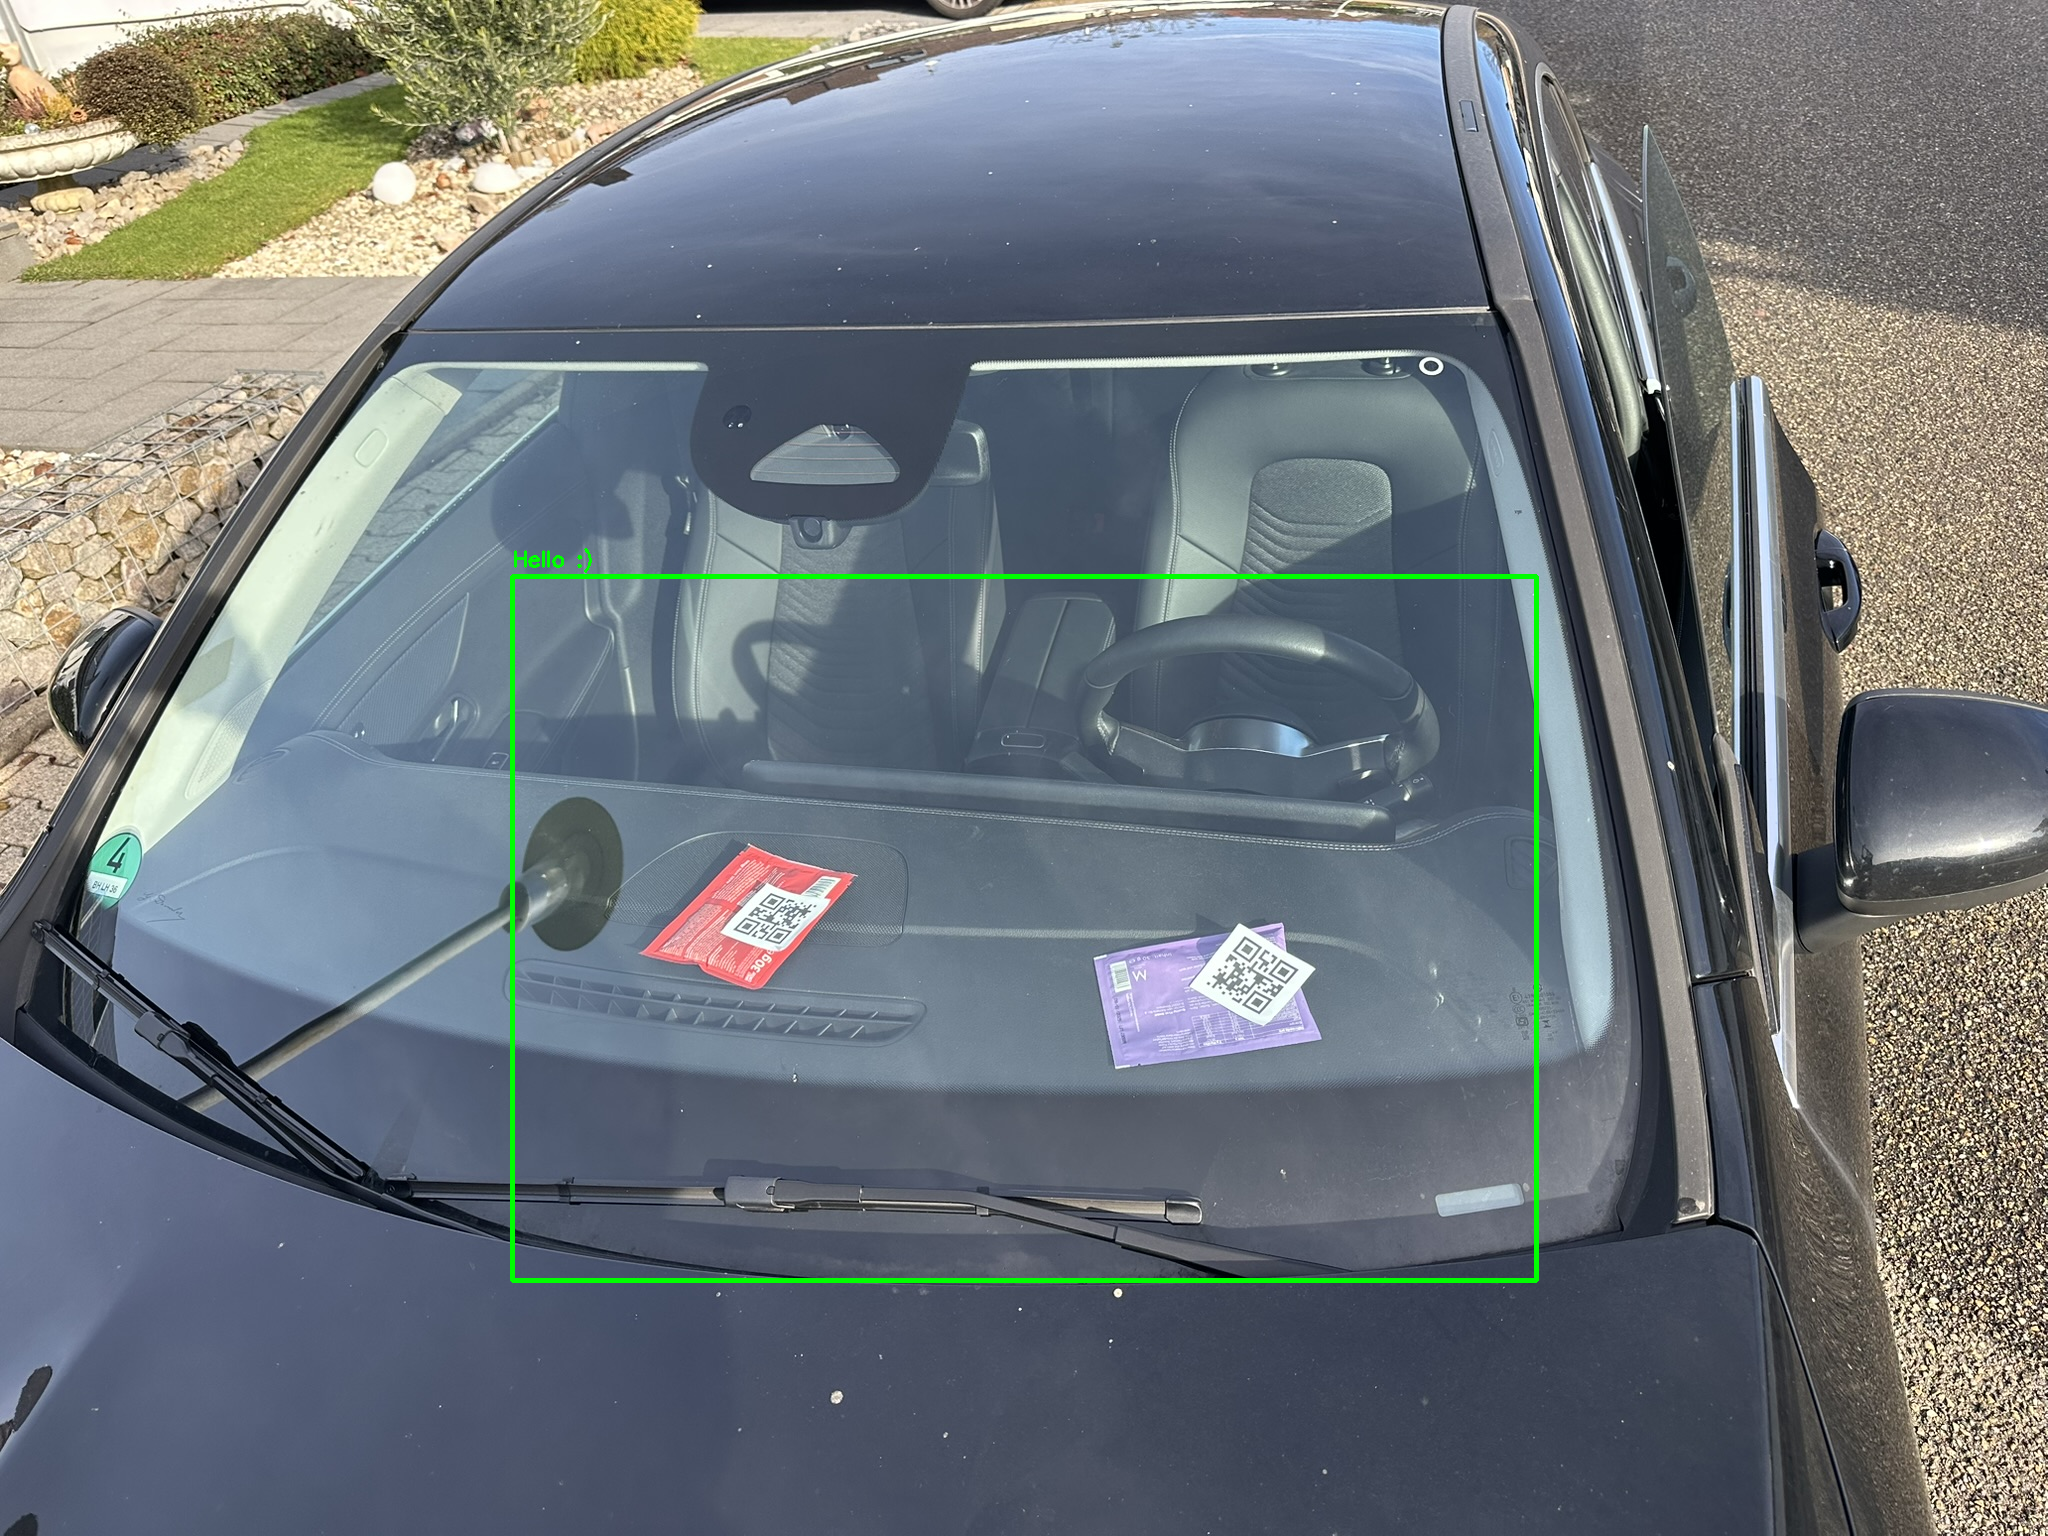
\includegraphics[width=0.8\textwidth]{Entcoded.PNG}
    \caption{Darstellung des entschlüsselten QR-Codes}
    \label{fig:final_decision}
\end{figure}

\subsubsection{Datensicherung und Log-File-Struktur}

Die Ergebnisse werden für die statistische Auswertung in einer semikolon-separierten Textdatei (\texttt{scan\_results.txt}) protokolliert. Dieses Format erlaubt sowohl eine einfache maschinelle Weiterverarbeitung (z.\,B. in Excel oder Python Pandas) als auch eine schnelle manuelle Kontrolle. Die Struktur folgt dem Schema:

\begin{center}
    \texttt{Dateiname;Status;Inhalt}
\end{center}

Ein konkreter Protokolleintrag für eine erfolgreiche Detektion stellt sich wie folgt dar:

\begin{lstlisting}[caption={Beispielhafter Eintrag in der Log-Datei}, frame=single]
IMG_7446.PNG;OK;Hello :)
\end{lstlisting}

Ein Bild wird logisch als \textbf{Erfolg (success)} eingestuft, sofern mindestens ein Code gelesen werden konnte. In diesem Fall wird für jeden gefundenen Inhalt eine eigene Zeile im Log generiert. Nur bei vollständiger Unlesbarkeit aller detektierten Bereiche erfolgt eine Einordnung als \textbf{failed}. Diese Struktur erlaubt eine präzise spätere Analyse der Erkennungsraten unter variierenden Umweltbedingungen, da der Status \texttt{OK} direkt mit dem extrahierten Datenstring korreliert.


% ==============================================================================
% KAPITEL 7: GEOMETRISCHE ANALYSE UND WINKELBERECHNUNG
% ==============================================================================
\section{Geometrische Analyse und Winkelberechnung}

Nach der erfolgreichen Detektion und Dekodierung der QR-Codes besteht die finale Zielsetzung darin, eine präzise Stellgröße für die Schwenkhardware der Kamera zu ermitteln. Dieser Prozess erfordert den Übergang von der zweidimensionalen Bildbetrachtung in eine dreidimensionale räumliche Analyse, um eine optimale Erfassungsgeometrie für den Einsatz in der Waschanlage zu gewährleisten.

\subsection{Methodik: Pose Estimation via SolvePnP}

Zur Bestimmung der räumlichen Orientierung des QR-Codes relativ zur Kamera wird das \textit{Perspective-n-Point} (PnP) Verfahren eingesetzt. Da ein QR-Code eine bekannte, quadratische Geometrie aufweist, lässt sich die perspektivische Verzerrung innerhalb des zweidimensionalen Abbilds mathematisch nutzen, um auf die Neigung der Oberfläche im Raum zurückzuschließen.

Das Verfahren basiert auf dem Abgleich zweier Koordinatensysteme:
\begin{itemize}
    \item \textbf{3D-Modellraum (Weltkoordinaten):} Definition des QR-Codes als ideales, flaches Quadrat im virtuellen Raum (z.\,B. Koordinaten von -5,0 bis +5,0 Einheiten).
    \item \textbf{2D-Bildraum (Pixelkoordinaten):} Die durch die KI detektierten vier Eckpunkte des verzerrten Polygons innerhalb des Kamerabildes.
\end{itemize}

Mittels der mathematischen Funktion \texttt{cv2.solvePnP} wird die Rotation und Translation berechnet, aus welcher der \textbf{Pitch-Winkel} (Neigung um die X-Achse) extrahiert wird. Dieser Winkel repräsentiert die Abweichung zwischen der aktuellen optischen Achse der Kamera und der Normalen (der Senkrechten) der QR-Code-Ebene.

\subsection{Differenzierung der Winkel-Kategorien}

Für die korrekte Interpretation der Ergebnisse ist eine strikte Unterscheidung zwischen zwei Winkeldefinitionen essenziell:

\subsubsection{Der relative Tilt-Winkel (Bildspezifische Messung)}
Dieser Wert wird für jedes analysierte Bild individuell berechnet. Er beschreibt die verbleibende Abweichung zur idealen Draufsicht in einer spezifischen Aufnahme. Ein Messwert von \SI{0}{\degree} würde bedeuten, dass die Kamera bereits perfekt orthogonal (im $90^\circ$-Winkel) zum Code steht. Geringe Werte in den Testreihen, wie beispielsweise \SI{2,2}{\degree}, belegen, dass die Kamera zum Zeitpunkt der Aufnahme bereits nahezu ideal zum Zielobjekt ausgerichtet war.

\begin{figure}[H]
    \centering
    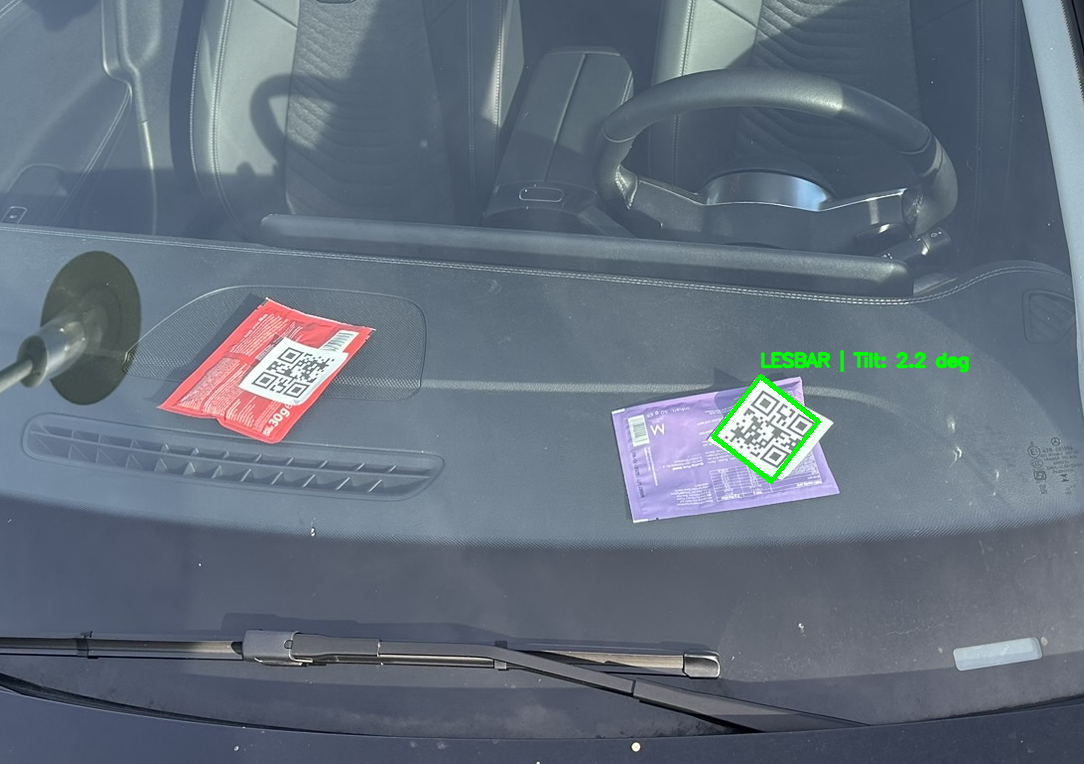
\includegraphics[width=0.8\textwidth]{tilt_winkel.PNG}
    \caption{Einzelbild-Analyse mit Angabe der relativen Winkelabweichung.}
    \label{fig:einzel_tilt}
\end{figure}

\subsubsection{Der absolute Montage-Winkel (Systemweite Empfehlung)}
Dieser Winkel bezieht sich auf die hardwareseitige Installation der Anlage. Ausgehend von einer horizontalen Grundstellung (Kamera blickt parallel zur Decke) definiert dieser Wert den notwendigen Schwenk nach unten, um den statistischen Durchschnitt der Fahrzeuggeometrien optimal abzudecken.

\subsection{Statistische Auswertung und Ergebnisse}

Um eine belastbare Montageempfehlung auszusprechen, wurde eine Großzahlanalyse über insgesamt 1075 erfolgreich dekodierte Datensätze durchgeführt. Die statistischen Kennzahlen dieser Untersuchung sind in der folgenden Tabelle zusammengefasst:

\begin{table}[H]
    \centering
    \caption{Statistische Kennzahlen der Winkelanalyse (Datengrundlage $n=1075$)}
    \label{tab:winkel_stats}
    \begin{tabular}{l l}
        \toprule
        \textbf{Parameter} & \textbf{Wert} \\
        \midrule
        Minimaler gemessener Winkel & \SI{0,0}{\degree} \\
        Maximaler gemessener Winkel & \SI{68,2}{\degree} \\
        Arithmetisches Mittel (Mean) & \SI{39,5}{\degree} \\
        \textbf{Median (Empfohlener Montage-Winkel)} & \textbf{\SI{44,3}{\degree}} \\
        \bottomrule
    \end{tabular}
\end{table}
Die Entscheidung für den Median als primäre Kenngröße für die Montageempfehlung gegenüber dem arithmetischen Mittel (Mean) begründet sich durch dessen statistische Robustheit. Während das arithmetische Mittel empfindlich auf Extremwerte reagiert – etwa bei vereinzelten Messungen von außergewöhnlich flachen Sportwagen oder sehr hohen Nutzfahrzeugen, bleibt der Median von solchen Ausreißern unbeeinflusst. 

Da die Datengrundlage eine hohe Varianz an Fahrzeugtypen abdeckt, deutet die Differenz zwischen dem Mittelwert (\SI{39,5}{\degree}) und dem Median (\SI{44,3}{\degree}) auf eine asymmetrische Verteilung der Messdaten hin. Der Median repräsentiert in diesem Kontext den Wert, der die Verteilung exakt halbiert, und liefert somit eine stabilere Stellgröße für die mechanische Ausrichtung. Durch die Wahl des Medians wird sichergestellt, dass die Kamera für die Mehrheit der in der Waschanlage vorkommenden Standard-Fahrzeuge eine nahezu ideale orthogonale Sichtachse einnimmt, ohne durch seltene Randfälle verzerrt zu werden.

\subsection{Wissenschaftliche Begründung der Montageempfehlung}

Die ermittelte Empfehlung von ca. \SI{44}{\degree} erscheint zunächst kontraintuitiv, wenn man eine rein horizontale Lage des QR-Codes auf dem Armaturenbrett unterstellt. Dennoch ist dieser Winkel aus physikalischer und praktischer Sicht einer $90^\circ$-Montage (senkrecht nach unten blickend) vorzuziehen:

\begin{enumerate}
    \item \textbf{Prävention von Totalreflexionen:} Eine senkrechte Sichtachse zur Windschutzscheibe würde bei Glasoberflächen zu starken Spiegelungen. beispielsweise der Deckenbeleuchtung, direkt zurück in das Objektiv führen. Durch den gewählten Schwenkwinkel von \SI{44,3}{\degree} werden Reflexionen nach dem physikalischen Prinzip „Einfallswinkel gleich Ausfallswinkel“ am Sensor vorbeigeleitet, was die Lesbarkeit massiv erhöht.
    \item \textbf{Geometrie der Erfassungsdistanz:} Das System muss Codes aus Entfernungen von bis zu \SI{3}{\meter} vor dem Fahrzeug erfassen. Eine schräge Blickrichtung ist hierfür notwendig, da bei einer $90^\circ$-Montage das Fahrzeugdach die Sicht auf das Armaturenbrett verdecken würde, bevor der QR-Code den Sichtbereich der Kamera erreicht.
    \item \textbf{Fahrzeugergonomie:} QR-Codes folgen meist der Neigung der Windschutzscheibe (typischerweise \SI{30}{\degree} bis \SI{55}{\degree}) oder liegen auf gewölbten Armaturenbrettern. Der Median von \SI{44,3}{\degree} bildet den empirischen „Sweet Spot“, um über eine maximale Varianz an Fahrzeugtypen hinweg eine nahezu orthogonale Projektion zu erzielen.
\end{enumerate}

\begin{figure}[H]
    \centering
    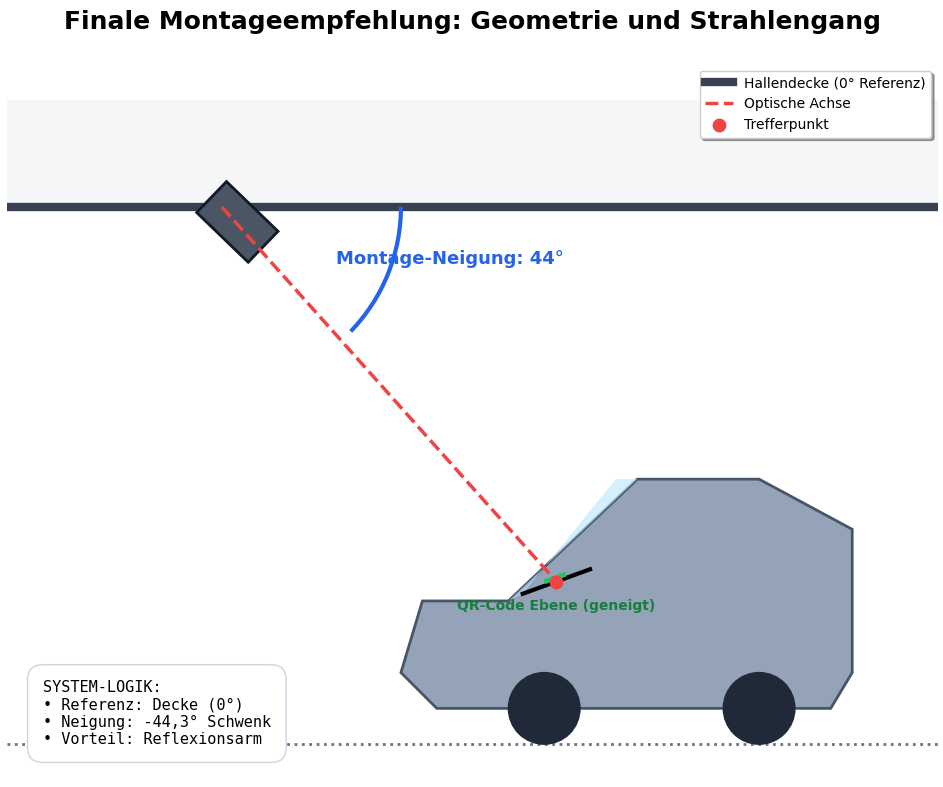
\includegraphics[width=0.8\textwidth]{globale_Winkelempfehlung.png}
    \caption{Schematische Darstellung der Montageempfehlung}
    \label{fig:montage_schema}
\end{figure}
% ==========================================
% ANHANG (Optional)
% ==========================================
%\newpage
%\appendix
%\section{Quellcode}
%\section{Datenblätter}

\end{document}